\FloatBarrier
\subsection{Filter cavities}\label{app:filtercavities}

The necessity of filter cavities for a broadband quantum noise reduction with a squeezed state of light was described in Secs.~\ref{sec:filtercavities} and App.~\ref{app:QNR}. In the following sections, the technical requirements for these optical filters are discussed. An important point is the required baseline length of these filter cavities in view of their optical round-trip loss (App.~\ref{app:FClength}). The tolerances of the determined design parameters will be discussed in App.~\ref{app:robustparam}. Furthermore, in App.~\ref{app:scatter} the optical layout with regard to the round-trip loss that will be mainly caused by scattering by the mirror surface defects is treated. Finally, the degradation of the squeezing level due to noise couplings (e.g.\ displacement noise in the filter cavities) will be analysed in Sec.~\ref{app:phsnoise}, leading to further estimates for the requirements.

\FloatBarrier
\subsubsection{Restrictions for the baseline length of the filter cavity}\label{app:FClength}

In this Section we start with a description of the influence of optical round-trip loss on the filter cavities performance in dependence of their baseline length and half-bandwidth. The required half-bandwidth $\gamma_{\rm fc}$ and detuning
$\Phi_{\rm fc}$ (note that we will define them as angular
frequencies) of the filter cavities giving the optimal frequency-dependent squeezing angle are determined by the interferometer
configuration and its induced phase-space rotation of light fields
entering the interferometers output port.

Generally, any round-trip loss will degrade the squeezing level at
sideband frequencies being resonant in the filter cavity (cf. Sec.~\ref{sec:filtercavities}). For a
given power round-trip loss $l^2_{\rm rt,fc}$
 (mainly caused by
scattering)  the resulting loss in reflection of the filter cavity
increases with a decreasing baseline length $L_{\rm fc}$
 of the
filter. As well, for a certain length  $L_{\rm fc}$ and a certain
round-trip loss $l^2_{\rm rt,fc}$ the loss imposed on the squeezed
field increases with a decreasing half-bandwidth $\gamma_{\rm fc}$
that needs to be realized.

Starting from the expression for the
half-bandwidth of a lossy cavity
\begin{equation} \gamma_{\rm fc} = \frac{c}{2 L_{\rm fc}}
\arccos\left(1-\frac{(1-\rho_{\rm c}\sqrt{1- l^2_{\rm
rt,fc}})^2}{2\rho_{\rm c}\sqrt{1- l^2_{\rm
rt,fc}}}\right)\,\label{eq:gamma}
\end{equation}
one can derive the filter cavity's coupling mirror power reflectance
$R_{\rm c}=\rho_{\rm c}^2$
 that is required to achieve the
targeted half-bandwidth. One obtains
\begin{equation}
\rho_{\rm c} = \frac{1}{\sqrt{1- l^2_{\rm
rt,fc}}}\left[2-\cos(\mathcal{F}^\prime) -
\sqrt{\cos^2(\mathcal{F}^\prime)-4 \cos(\mathcal{F}^\prime)+3}
\right]\label{eq:rc}
\end{equation}
with
\begin{equation}
\mathcal{F}^\prime =  \frac{2 \gamma_{\rm fc} L_{\rm fc}}{c} =
\frac{\gamma_{\rm fc}}{{\rm FSR_{fc}}}
=\frac{\pi}{\mathcal{F}_{\rm fc}}\,.
\end{equation}

\begin{figure}
\centering
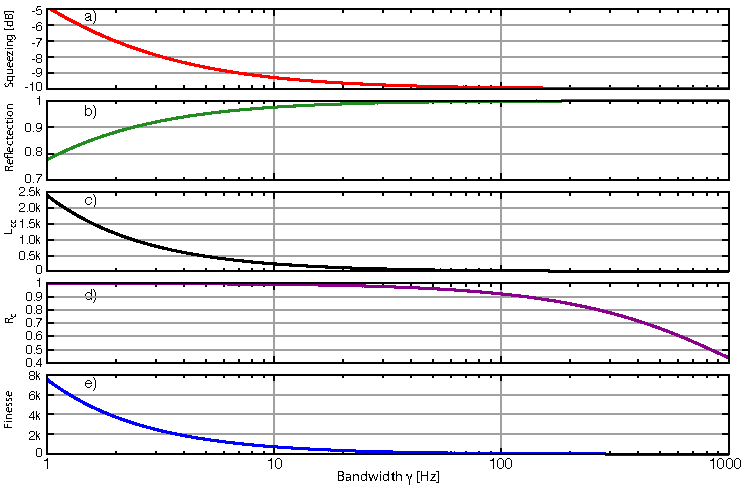
\includegraphics[scale = 1.2]{./Sec_Optics/FCsgammaAI75ppm.pdf}
\caption{Filter cavity properties in dependence of its half-bandwidth $\gamma_{\rm fc}$.  a) the remaining detectable squeezing level in reflection of the filter cavity and b) its reflectance at the frequency $\Omega =  \Phi_{\rm fc}L_{\rm fc}/c$. In c) the value for $L_{\rm cc}$ is shown according to Eq.~(\ref{eq:lcc}).  Curve d) shows the finesse and e) the coupling mirror reflectance $R_{\rm c}$ given by Eq.~(\ref{eq:rc}). For all traces a filter cavity length $L_{\rm fc}=10\,{\rm km}$ and a round-trip loss $l_{\rm rt,fc}^2=75\,{\rm ppm}$ was assumed. An initial pure 10\,dB squeezed state was considered. It can be seen that the impact of the round-trip loss becomes significant for $\gamma_{\rm fc}<2\pi\cdot10\,{\rm Hz}$.} \label{fig:gamma}
\end{figure}

Graph e) in Fig.~\ref{fig:gamma} shows the value for $R_{\rm
c}=\rho_{\rm c}^2$ according to Eq.~(\ref{eq:rc}). In the
underlying calculations the baseline length $L_{\rm fc}$ and the
round-trip loss $l_{\rm rt,fc}^2$ were considered with 10\,km and
75\,ppm, respectively.  The tuning of the filter cavity was
exemplary set to $\Phi_{\rm fc}=\gamma_{\rm fc}L_{\rm fc}/c$. It
can be seen, that for small half-bandwidths $\gamma_{\rm fc}$ the
reflectance  $R_{\rm c}$ comes close to unity.  Correspondingly,
the resulting finesse rises as shown in Graph d). It can be seen
from Eq.~(\ref{eq:rc}) that there are two fundamental restrictions
for the choice of the filter cavity length. First, for great
values of the finesse (i.e.\ for small half-bandwidths) we obtain
\begin{equation}
\lim_{\gamma_{\rm fc} \to 0} \rho_{\rm c} = \frac{1}{\sqrt{1-l_{\rm rt,fc}^2}}> 1
\end{equation}
which does not represent a physical solution. Thus, there must
exist a value $L_{\rm min}$ such that for $L_{\rm min} < L_{\rm
fc}$ we always have $\rho_{\rm c}<1$. The expression for $L_{\rm
min}$ can be derived to
\begin{equation}
L_{\rm{min}} =
\frac{c}{2\gamma_{\rm{fc}}}\arccos\left[2-\frac{2-l_{\rm{rt,fc}}^2}{2\sqrt{1-l_{\rm{rt,fc}}^2}}\right]\,.
\end{equation}

Second, for $L_{\rm fc} < L_{\rm cc}$ we obtain $\rho_{\rm
c}>\sqrt{1-l_{\rm rt,fc}^2}$ and the filter cavity becomes
under-coupled. But even in the most general case, the
interferometer represents an over-coupled cavity. Hence, an
under-coupled filter cavity with $L_{\rm fc} < L_{\rm cc}$ can not
provide the phase-space rotation required for the generation of
the optimal squeezing angle.

To keep  $\rho_{\rm c}<\sqrt{1-l_{\rm rt,fc}^2}$ the filter cavity length needs to be
\begin{equation}
L_{\rm fc} > L_{\rm cc} =
\frac{c}{2\gamma_{\rm{fc}}}\arccos\left[2-\frac{1+(1-l_{\rm
rt,fc}^2)^2}{2(1-l_{\rm rt,fc}^2)}\right]\label{eq:lcc}
\end{equation}
Note that for $L_{\rm fc}=L_{\rm cc}$ the filter cavity is
critically coupled (impedance matched) and the loss in its
reflection is maximum. Therefore, to preserve the squeezing in
reflection of the filter cavities its length should be chosen with
$L_{\rm fc} \gg L_{\rm cc}$. This fact becomes obvious when
looking at graph a) and b) of Fig.~\ref{fig:gamma}. They show the
squeezing level in reflection of the filter cavity and the according reflectance of the filter cavity at its resonance frequency, respectively. At small half-bandwidths the
value for $L_{\rm cc}$ (graph c)) is of the order of the filter
cavity's baseline length $L_{\rm fc}=10\,{\rm km}$ and hence the reflectance
and accordingly the remaining squeezing level are considerably
reduced.

In Fig.~\ref{fig:length_maintext} the filter cavity performance is shown
depending on its baseline length $L_{\rm fc}$. In the
corresponding calculations we assumed the target half-bandwidth
with ${\gamma_{\rm fc} = 2\pi\cdot1.4\,{\rm Hz}}$ and the target detuning with
${\Phi_{\rm fc_1}= 2\pi\cdot 6.6\,{\rm Hz}\cdot L_{\rm fc_1}/c}$.
Note, that these values are approximately the requirements for one of the filter
cavities that needs to be realised in the ET-LF
detector~\cite{Hild2010a}. Again, the round-trip loss was
considered of 75\,ppm and the initial squeezing level of 10\,dB.  Graph a)
demonstrates, that even with a filter cavity length of 10\,km the
amount of squeezing  is already reduced by a factor of about
4\,dB. For lengths smaller than about 2.5\,km the unbalanced loss for upper and lower squeezing sidebands results in a noise enhancement (anti-squeezing) when compared to vacuum noise in reflection of the filter cavity.  At the critical length $L_{\rm fc} = L_{\rm
cc}\approx1239\,\rm m$ this enhancement becomes maximum and corresponds to about 5\,dB anti-squeezing. For lengths smaller than $L_{\rm cc}$  the noise level drops and squeezing can be achieved again (grey shaded area~II) until it reaches at $L_{\rm fc} =
L_{\min}$ the initial level of 10\,dB. However, in this region the
filter is under-coupled and does not yield the required
phase-space rotation of the squeezed field. This can be understood
when considering the extreme case for $L_{\rm fc} = L_{\min}$.
Here, $R_{\rm c}$ is equal to one and  the filter cavity can be
replaced by  an ordinary mirror that has no frequency dependence.
Again, it can be deduced that a filter cavity length  $L_{\rm fc}
\gg L_{\rm cc}$ needs to be realised in order to preserve the
squeezing. In addition, the high finesse of a short cavity might
pose a problem for the lock acquisition in the environment of a gravitational-wave detector where the optics
needs to be suspended.

So far in Figs.~\ref{fig:gamma} and~\ref{fig:length_maintext} the squeezing level was shown in reflection of the considered filter cavities at its resonance frequency. Here the  (frequency-dependent) imposed loss is maximum. Now, for  exemplification
Fig.~\ref{app:fig:sqz} shows squeezing spectra obtained after the
reflection at two subsequent filter cavities FC$_1$ and FC$_2$.

The considered  half-bandwidths and tunings of these filters are
those needed for the ET-LF detector. The length of the cavities
were considered with  $L_{\rm fc_1}=L_{\rm fc_2}=2\,{\rm km}$ (red
curve), $L_{\rm fc_1}=L_{\rm fc_2}=5\,{\rm km}$ (blue curve) and
$L_{\rm fc_1}=L_{\rm fc_2}=10\,{\rm km}$ (green curve),
respectively.


The calculations and exemplary filter properties considered within
this Section imply that in 3rd generation gravitational-wave
detectors such as the Einstein Telescope, where filter cavities with half-bandwidths
in the range of ${\gamma_\text{fc}\approx 2\pi\cdot1- 2\pi\cdot5\,\mathrm{Hz}}$ will be
required, the baseline length of these filters needs to be in the
order of a few kilometers. This contrasts to the results presented
in \cite{Khalili2009} for the Advanced LIGO
detector. As for the Advanced LIGO configuration filter cavities with
half-bandwidths in the order of ${2\pi\cdot50- 2\pi\cdot200\,{\rm Hz}}$ will be required, a
considerable sensitivity increase by the injection of frequency-dependent squeezed light can already be achieved if filter
cavities with lengths in the order of 100\,m are utilised. Certainly,
our exemplary calculations are based on a conservative assumption
of 75\,ppm for the round-trip loss of the filter cavities, but
even if optimistic values of $l_{\rm rt,fc}^2=20\,\mathrm{ppm}$ are
considered, the corresponding values for the critical lengths will
be $L_{\rm cc, fc_1} = 330\,{\rm m}$ and  $L_{\rm cc, fc_2} =
84\,{\rm m}$, respectively. As shown in Figs.~\ref{fig:gamma}
and \ref{fig:length_maintext} the respective length $L_{\rm fc}$ should be
at least 10 times greater than $L_{\rm cc}$.   I.e.\ for the ET-LF detector the  length of the two required filter cavities should be 10\,km. In contrast, it can be shown that for the ET-HF detector a filter with a length of about 500\,m is sufficient. This filter will be required for an optimisation of the squeezed quadrature in the radiation pressure noise dominated frequency band. However, in this frequency band other noise sources dominates the quantum noise. For that it is satisfactory to adapt the squeezing level to the level of these noise sources which will be possible with a comparatively short filter cavity.



The former investigation demonstrated that  the round-trip loss ultimately restricts the minimal allowed baseline length and consistently the performance of the filter cavities. As it is expected that the round-trip loss of the filters will be dominated by scattering at imperfect mirror surfaces, the optical layout needs to be designed such that the amount of scattering is as much as possible reduced. The scattering in different optical layouts is treated in Sec.~\ref{subsec:fcscattering}.

\begin{figure}
\centering
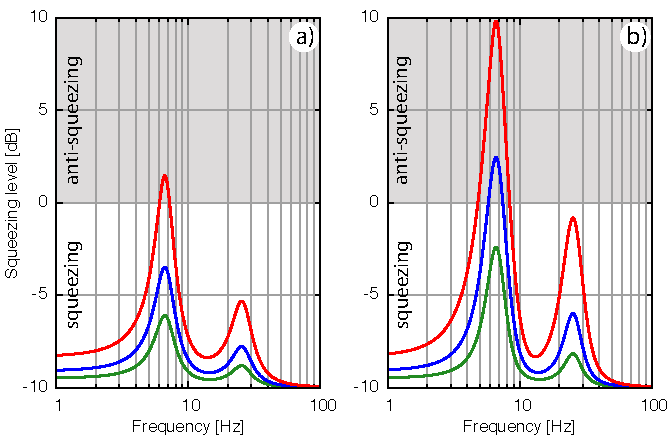
\includegraphics[scale = 1.2] {./Sec_Optics/ET-C-FiltersAI.pdf}
\caption{The figure shows the remaining squeezing level after subsequent reflection at two filter cavities FC$_1$ and FC$_2$. In graph~a) an initial pure 10\,dB squeezed state was considered and 75\,ppm round-trip loss in each cavity. Additionally, in graph~b)  optical loss of 9\,\% outside the filter cavities was considered. Thus, an initial pure 20\,dB squeezed state is necessary to achieve 10\,dB detectable squeezing. In both cases, three length of the cavities were considered. The green curves are obtained for $L_{\text{fc}_1}=L_{\text{fc}_2}=10\,\mathrm{km}$, the blue one for  $L_{\text{fc}_1}=L_{\text{fc}_2}=5\,\mathrm{km}$ and the red one for  $L_{\text{fc}_1}=L_{\text{fc}_2}=2\,\mathrm{km}$. The filter parameters are approximately those that are required for a broadband quantum noise reduction in the ET-LF detector, i.e.\ $\gamma_{\text{fc}_1}=2\pi\cdot1.4\,\mathrm{Hz}$, $\Phi_{\text{fc}_1}= 2\pi\cdot6.6\,\mathrm{Hz}\cdot L_{\text{fc}_1}/c$ and $\gamma_{\text{fc}_1}=2\pi\cdot5.7\,\mathrm{Hz}$, $\Phi_{\text{fc}_1}= -2\pi\cdot25.4\,\mathrm{Hz}\cdot L_{\text{fc}_1}/c$, respectively. Please note, that from this comparison it can be deduced, that the tolerable loss in the filters needs to be determined also in view of the injected anti-squeezing.}
\label{app:fig:sqz}
\end{figure}
\FloatBarrier
\subsubsection{Determination of the required filter parameters}\label{app:detfcparams}

In publications by Purdue and Chen~\cite{Purdue2002a} and Harms \cite{OpticalSpringHarms2003} treating the frequency dependent squeezed light injection, some analytical expressions were derived showing first the need for filter cavities and second allow for a calculation of the required number,  bandwidth and tuning of filter cavities.
In these works the interferometer quantum noise transfer function was derived using the Caves-Schumacher two-photon formalism~\cite{Caves1985}. The interferometer quantum noise transfer function is then described by a $2\times 2$-matrix $\mathbf{T}$ (refer to Eq.~(3) in \cite{OpticalSpringHarms2003}).  From this matrix the required frequency-dependent squeezing angle $\lambda(\Omega)$ can be derived according to Eq.~(16) in \cite{OpticalSpringHarms2003}

\begin{equation}
\lambda(\Omega) = \arctan\left(-\frac{T_{11}\cos\zeta + T_{21}\sin\zeta}{T_{12}\cos\zeta + T_{22}\sin\zeta}\right)\,.\label{eq:lopt}
\end{equation}

Here, $\Omega$ is the angular sideband frequency and $\zeta$ the read-out angle. It was shown in \cite{Purdue2002a}, that with a combination of Fabry-Perot cavities the required frequency dependent angle $\lambda(\Omega)$ can be realized. It  has the form \cite{Purdue2002a}
\begin{equation}
\tan\lambda(\Omega) = \frac{\sum_{k=0}^{n} B_k\Omega^{2k}}{ \sum_{k=0}^{n} A_k\Omega^{2k}}\,, \text{with}\, \left|A_n+\mathrm{i}B_n\right|>0
\end{equation}

From the corresponding characteristic equation
\begin{equation}
\sum_{k=0}^{n} \left(A_k+\mathrm{i}B_k\right)\Omega^{2k}=0\label{eq:chareq}
\end{equation}
the required bandwidth and tuning of the filter cavities can be obtained. They are given by the $2n$ roots (in $n$ pairs with a positive imaginary part) of Eq.~(\ref{eq:chareq}).
However, these calculations are based on the assumption of a lossless main interferometer, an infinite small signal-recycling cavity length,  an expansion in powers of the light's angular frequency and the approximated expression for a cavity's half-bandwidth $\gamma=c\tau_{\rm c}/(4L)$. Thus, in general they allow just for a precise estimation for the required parameters.

Furthermore it is demonstrated in Fig.~\ref{fig:phs-vs-loss}, that it is not sufficient to realize filter cavities having the bandwidth and tuning determined by Eq.~(\ref{eq:chareq}).   First, the impact of optical loss was considered. Therefore, the phase-space rotation in reflection of a cavity with a half-bandwidth $\gamma=2\pi\cdot1.44448\,\rm Hz$ and a tuning according  to $f_{\rm res} = 6.628\,\rm Hz$ is calculated for different values of the round-trip loss. The length was set to 10\,km. The results are shown in the left graph of Fig.~\ref{fig:phs-vs-loss}. It can be seen that the deviation of the phase-space rotation related to the lossless case increases with increasing optical loss. Similarly, the rotation in reflection depends on the baseline length of the cavity. This fact is shown in the right graph of Fig.~\ref{fig:phs-vs-loss}. Here, the round-trip loss was set to 75\,ppm for all cases.


 \begin{figure}
 \centering
   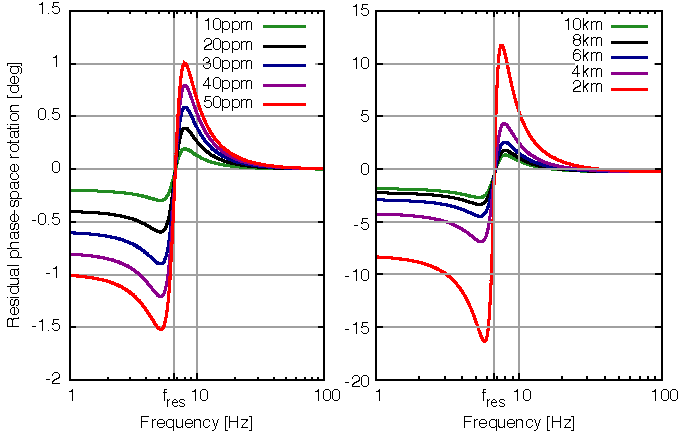
\includegraphics{./Sec_Optics/PhsRot-residualsAI.pdf}
   \caption{The figure demonstrates, that the phase-space rotation of a Fabry-Perot cavity is not only determined by its resonance frequency and bandwidth (here exemplary set to 6.628\,Hz and 1.44448\,Hz, respectively, for all cases), but also by its round-trip loss (left for a length of 10\,km) and its baseline length (right for losses of 75\,ppm).}
   \label{fig:phs-vs-loss}
   \end{figure}


Especially under consideration of optical intra-cavity round-trip loss and a finite baseline length of the filter cavities as well as the signal-recycling cavity,
there is no possibility to determine the optimal filter cavities parameters analytically. Thus, the parameters for the filter cavities were fitted with respect to the residual phase-space rotation of injected squeezed field. Fig.~\ref{fig:phs-fit-75ppm} compares the results for the parameters determined in accordance to Eq.~\ref{eq:chareq} (red curve) and those determined by the fit (black curve) for the ET-D LF detector. The corresponding filter cavity parameters are listed in Tab.~\ref{tab:ETDLFfitanaparamsloss}

\begin{figure}
 \centering
   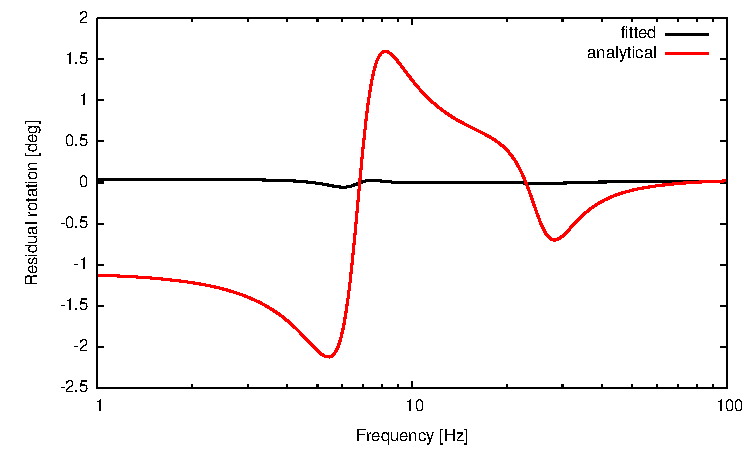
\includegraphics{./Sec_Optics/Fit_realparams.pdf}
   \caption{The figure shows the residual rotation of the injected squeezing, if the filter cavities are realized with parameters determined in accordance to Eq.~(\ref{eq:chareq}) (red curve) and those determined by  a fit (black curve). After fitting the parameters, the residual rotation is less than 0.2 deg.}
   \label{fig:phs-fit-75ppm}
   \end{figure}


\etbox{i}{rbox:fcparam}{Determination of the required filter parameters}
{\begin{table}[H]
\centering
\color{\contentcolor}
\begin{tabular}{c|c|c}
\hline
\hline
 & tuning [Hz]  (fitted / analytical) & half-bandwidth [Hz] (fitted / analytical)\\
\hline
FC$_1$ &-25.4255 / -25.3592  & 5.76766 / 5.68148\\
FC$_2$ & 6.6167 / 6.6280  & 1.53135 / 1.44448  \\
\hline
\hline
\end{tabular}
\caption{Deduced design parameters for the ET-D LF Filter-cavities.}
\label{tab:ETDLFfitanaparamsloss}
\end{table}
\begin{table}[H]
\centering
\color{\contentcolor}
\begin{tabular}{c|c|c}
\hline
\hline
 & tuning [Hz]  (fitted / analytical) & half-bandwidth [Hz] (fitted / analytical)\\
\hline
FC$_1$ &-- / -25.3592  & -- / 5.68148\\
\hline
\hline
\end{tabular}
\caption{Deduced design parameters for the ET-D HF Filter-cavities.}
%\label{tab:ETHFfilterparams}
\end{table}
}

\FloatBarrier
\subsubsection{Robustness of the design parameters}\label{app:robustparam}
In this section we illustrate the effect of a deviation from the determined design parameters. We will concentrate on the most obvious quantities, that will potentially  change the properties of the filter, i.e.\

\begin{enumerate}
\item{the reflectance factors of the used mirrors, }
\item{the round-trip loss,}
\item{the macroscopic length, and}
\item{the resonance frequency.}
\end{enumerate}
The first three quantities affect the bandwidth of the filter cavity and thus the required phase-space rotation around the targeted resonance frequency. A deviation from the design values of these quantities could not be compensated if the filter cavity is realised as  single resonator. An adaption of the filters bandwidth would be possible if coupled resonators---e.g.\ a linearly coupled three-mirror cavity---are utilised.  Although it should be always possible to tune the filter cavity to the required resonance frequency, for the sake of completeness we treat a potential  mismatch within this section. From the results the requirements for the length stabilisation with regard to displacement noise could be determined.

We start from the set of design parameters for the length, the detuning and the mirror reflectance factors yielding the bandwidth and phase-space rotation of the two filter cavities that are required for ET-C LF. These parameters are listed  in Table~\ref{tab:designparams}. The analysis of the impact on the achievable squeezing levels for a certain mismatch of the bandwidths will give the allowable tolerances of theses parameters.
\begin{table}[h]
\begin{center}
\begin{tabular}{lcc}
\hline
\hline
Parameter & FC$_1$ & FC$_2$\\
\hline
length $L_{\rm fc}$ [km] & 10 & 10\\
half-bandwidth $\gamma_{\rm fc}$ [Hz] & $2\pi\cdot1.4$ & $2\pi\cdot5.7$\\
resonance frequency  $f_{\rm res}$ [Hz] &  $2\pi\cdot6.6$ & $-2\pi\cdot25.4$\\
detuning $\Phi_{\rm fc}$ [$^\circ$] & $\approx 0.1369$ & $\approx 0.3026$\\
round-trip loss $l_{\rm rt,fc}$  [ppm] &75  & 75\\
coupling mirror reflectance $R_{\rm c}$ & 99.8864\,\% & 99.5323\,\%\\
\hline
\hline
\end{tabular}
\end{center}
\caption{Design parameters / estimates for the two filter cavities FC$_1$ and FC$_2$ needed in the ET-C LF detector.}
\label{tab:designparams}
\end{table}


To demonstrate the effect of a mismatched bandwidth we calculate the squeezing spectra after reflection at two subsequent resonators-- the required filter cavity and an auxiliary cavity which models the interferometer. For the filter cavity the design parameters (and a certain deviation of them) as listed in Table~\ref{tab:designparams} are assumed. The auxiliary one has a bandwidth and detuning  that models the transfer function and thus the phase-space rotation of the interferometer.  Consistently,  no phase-space rotation occur after subsequent reflection at these resonators if their bandwidths are matched.   Note, that  the auxiliary resonator is assumed to be loss-free so that the imperfections in the squeezing spectra can be clearly traced back to the respective deviation of the filter cavities design parameters. For a first illustration of the effect of a mismatched filter cavity bandwidth, Fig.~\ref{fig:devBWll} shows the squeezing level (top) and the residual phase-space rotation (bottom) after subsequent  reflection at both cavities. Note that here  \emph{both} cavities  were assumed to be loss-free.



\begin{figure}
\centering
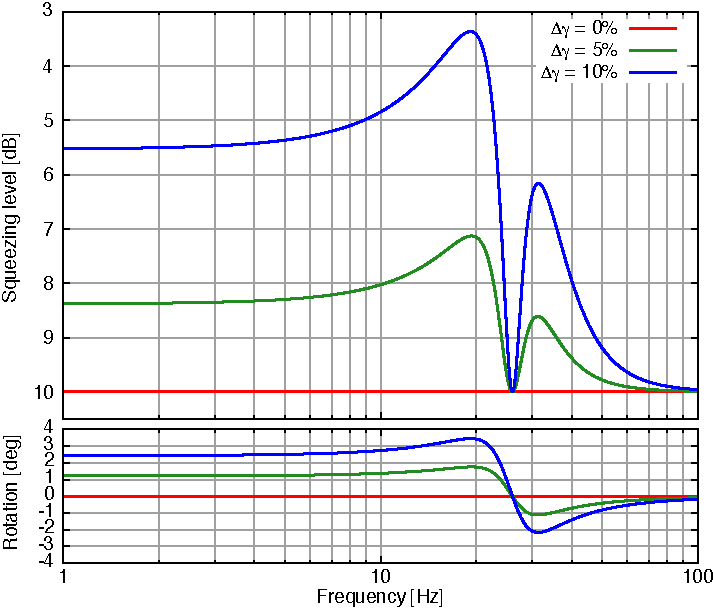
\includegraphics{./Sec_Optics/FCs-devbw-10-20-rotAI.pdf}
\caption{The figure illustrates the effect of a deviation of the required bandwidth. The lower graph shows the resulting residual phase-space rotation of the squeezing ellipse, the upper graph the according squeezing levels. Please note that the filter cavities are assumed to be lossless. Thus, the degradation of the squeezing level can be clearly traced back to the residual phase-space rotation.}
\label{fig:devBWll}
\end{figure}

Fig.~\ref{fig:devBW} shows the performance of the filter cavities
(FC$_1$ and FC$_2$)  required for the ET- LF detector. Their bandwidth
was varied according to a deviation of 1\,\% to 5\,\% from the
designed value. In these plots, the round-trip loss of the filter
cavities was considered to be 75\,ppm.

\begin{figure}
\centering
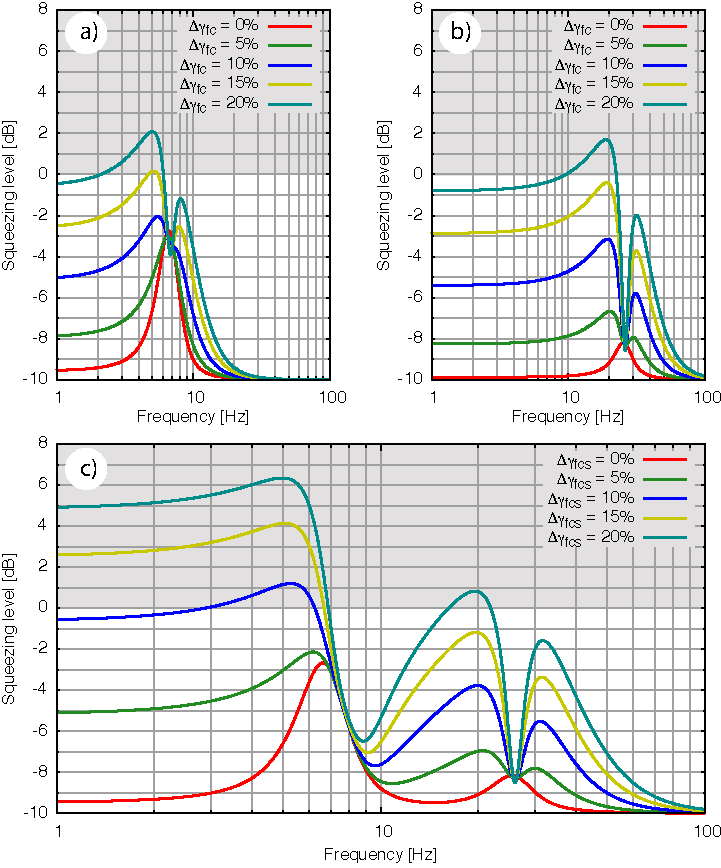
\includegraphics{./Sec_Optics/FCi-devbw_reviewAI.pdf}
\caption{The figure shows the squeezing spectra for a deviation of the designed bandwidth of a) the single FC$_1$  and b) the single FC$_2$. Graph c) shows the spectra if both  filter cavities are considered. In all cases, the filter cavity round-trip loss was considered to be 75\,ppm.}
\label{fig:devBW}
\end{figure}


\subsubsection{Scattering light noise in optical cavities}\label{app:scatter}
%\emph{Author(s): K Kokeyama, H. L\"{u}ck, A. Freise}

\begin{comment}
We have estimated the scattering between suspended mirrors for
different cavities geometries to determine whether this process
affects the selection of the geometry of the  ET filter cavities.

% scattering process
Deviations from a perfect mirror surface can scatter the main laser beam.
Scattered fields propagate along arbitrary spurious paths inside the cavity.
In general,  when the wavefront of the scattered light is changed
by deformations of the mirror surfaces,
the scattering into any direction is given by the Fourier transform of the mirror surface.
The longer spatial wavelengths presented in the mirror surface give smaller scattering angles.
A typical mirror surface has more long spacial wavelengths
than short spacial wavelengths, therefore, the scattering angle will be very small.

The scattered light propagates along spurious paths and reaches the detection port,
it couples to the main beam to create phase noise.
At the same time some scattered light fields may go out of the cavity and are lost.
This contributes to the optical loss, and the amount of the loss depends on the number of mirrors
in the cavity, and the mirror bidirectional distribution function (BRDF).
%
Here, we consider only the phase noise effect for this geometry analysis.

% Three scenarios
For the four cavity geometries, the following three scattering scenarios were considered:
\begin{itemize}
\item Direct back scattering.
When the main beam is reflected by a mirror, a part of the light field is scattered back
by the non-uniform distribution of the mirror surface.
% explain
Considering mirror angles, this effect is expected to be relatively small.
%The scattered field couples with the cavity resonant mode
%in the opposite direction in respect to the propagation direction of the main beam,
%just after being scattered by one mirror.
%%% small angle, large angle, special frequency of the mirror surface
 (triangular, rectangular, and bow-tie cavities)
%
%
\item Diagonal path scattering in a rectangular cavity.
In a rectangular cavity, when the main beam illuminates a mirror,
scattered light is emitted and propagates along the diagonal lines of the rectangular geometry.
After propagating along the diagonal path,
this field goes back into the cavity and reaches at the detection port,
resulting in the phase noise.
%
%
\item Gaussian tail effect.
In the rectangular and bow-tie cavities, the tail of the Gaussian field
may interact with the wrong mirror, for example as shown in Fig.~\ref{fig:Gtail1},
and is partially reflected. This reflected field couples into the main Gaussian beam.
\end{itemize}
\begin{figure}
\centering
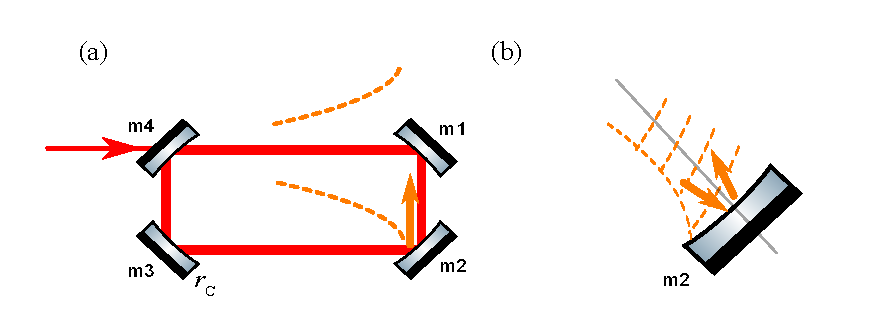
\includegraphics[width=0.7\textwidth]{./Sec_Optics/Gtail.pdf}
\caption{One exemplary path of (a) Direct back scattering.
This occurs at all mirrors except the linear cavity.
(b) Diagonal path scattering. This occurs only in the rectangular geometry.
(c) Gaussian tail effect. The rectangular or bow-tie cavities have this effect.
In addition to the exampled paths shown here, all the possible paths
were considered and summed to evaluate the scattering noise level.}
\label{fig:Gtail1},
\end{figure}

% Coupling factor
The convolution between the scattered field and the main beam was numerically calculated
to evaluate the coupling between the scattered field and the fundamental mode.
As the detailed optical parameters, such as the optimum beam sizes, are not fixed
for filter cavities yet, ET arm cavity parameters were used, e.g.,
the cavity length of 10 km and the mirror radius of 0.31 m.

% result and summary
The direct back scattering was found to be at a negligible scattering level.
This is because the wavefront of the scattered light is changed
when it is reflected by the angled mirror surface in all geometries,
and the wavefronts of the scattered light and the main field do not overlap or couple.
%
Additionally, this scenario is expected to be negligible
also because a typical mirror surface has more long spacial wavelengths
than short spacial wavelength, therefore,
most of the scattering occurs at much smaller angles than in this scenario
(for example the angle is 45 degrees in the rectangular cavity).
As mentioned above, a typical mirror surface has longer spacial wavelength components,
and the scattering angle due to this effect will be very small.

When the closer two long paths are separated by 1 m (between m1 and m2 in Fig~\ref{fig:Gtail1}),
The Gaussian tail effect is found to be negligible, as well.

One has to be careful when considering the scattering field propagating
along the diagonal paths in the rectangular cavity.
In order to block the diagonal paths, placing baffles
inside the rectangular geometry will be useful
to prevent the scattered light propagating along the base paths.

This analysis is also applicable to the ET arm cavities as well as
the filter cavities.
\end{comment}




We have estimated the amount of scattering in long baseline cavities
between the suspended optics for
different cavities geometries to test whether this particular class of scattering
has any influence on the selection of the optical resonator  for ET filter cavities.
The four cavity geometries depicted in Fig.~\ref{fig:new1} were considered.

% new version note
At the detection port, a photodetector detects the light field as
\begin{eqnarray}
P_{\rm out}=E E^*.
\end{eqnarray}
%
In addition to the cavity fundamental mode $E_c$,
we also consider a complex field $\delta E$ which occurs due to scattering,
thus we write
\begin{eqnarray}
E=E _c + \delta E.
\end{eqnarray}
The detected field is proportional to
\begin{eqnarray}
P _{\rm det} &\propto & (E _c + \delta E) (E_c^* +\delta E ^*)\\
&\propto & |E_c| ^2 + |\delta E| ^2 + E_c \delta E ^* + E _c ^* \delta E
\end{eqnarray}
where the first term is the power of the main mode,
and the second term is the power of the scattering filed
which is the second order term and assumed to be negligible.
Only the cross terms between the fundamental and complex scatter field
affects the sensitivity.
%
Considering the x-y plane, the cross term, or coupling factor, is written as
\begin{eqnarray}
\label{eq:couple}
X=\int ^{\infty} _{-\infty} \int ^{\infty} _{-\infty} E _c (x,y,z)
\delta E ^* (x,y,z) {\rm d}x {\rm d}y,
\end{eqnarray}
where
%$E _{\rm sc}(x,y,z_{\rm sc})$ is the scattered light field,
%$z_{\rm sc}$ is the location when the scattering  process occurs
the $z$ axis is the main beam propagation direction,
%and $z _{\rm cav}$ is the locations of the target field coupled by the scattered light.
and $E _{\rm cav}(x,y,z _{\rm cav})$ is the Gaussian field which is the resonant mode in the cavity,
%and the scattered field $\psi _{\rm sc}(x,y,z_{\rm sc})$ coupled into this mode:
\begin{eqnarray}
E _{\rm c}(x,y,z)=\sqrt{\frac{k_0}{\pi z_R}} \frac{i z_R}{z+i z_R}
\exp \biggl[ \frac{-i k_0 (x^2 +y^2)}{2(z+i z_R)} \biggr]
\end{eqnarray}
where $z_R$ is the Rayleigh range of the cavity resonant mode and $k_0$
is the wave number of the laser source.


\begin{figure}
\centering
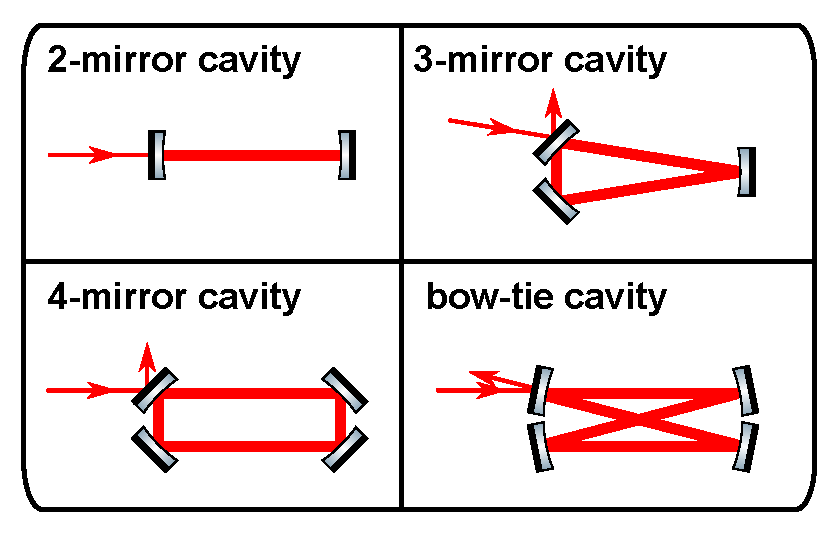
\includegraphics[scale =0.6]{./Sec_Optics/cavity-designs.pdf}
\caption{The scattering-light effects for four geometries,
(1) Two-mirror cavity, (2) triangular cavity, (3) rectangular cavity,
and (4) bow-tie cavity, are analysed.}
\label{fig:new1}
\end{figure}

\begin{figure}
\centering
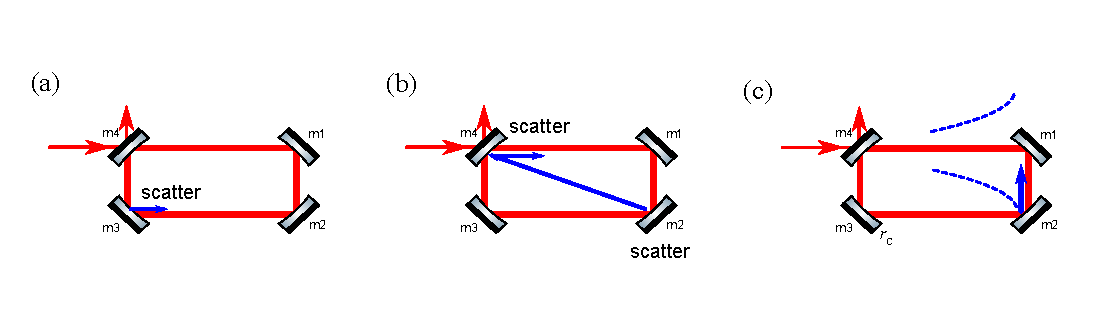
\includegraphics[scale =1]{./Sec_Optics/process.pdf}
\caption{Three scattering processes considered in this analysis.
(a) An exemplary field of the direct back scattering. It occurs at all mirrors
in each geometry except in the two-mirror cavity.
(b) Diagonal path scattering. In the rectangular cavity, the diagonal paths
in the rectangular geometry create spurious paths.
(c) Gaussian tail effect. In the rectangular and bow-tie cavities,
the tail of the Gaussian field may interact
with the wrong mirror, is partially reflected.
This reflected field couples into the main Gaussian beam. }
\label{fig:process}
\end{figure}


% how to evaluate
Here, we consider three simplified scenarios of scattering processes,
in order to estimate the scattered light levels in candidate ET cavities;
direct back scattering, diagonal path scattering,
and the Gaussian tail effect.
The three processes will be evaluated and compared between the four
cavity geometries:
a two-mirror cavity, triangular cavity, rectangular cavity, and bow-tie cavity,
as shown in Fig.~\ref{fig:new1}.

% coupling coefficient
%\subsection{Coupling factor}
%To evaluate the effect of the scattered light noise,
%we calculate how much the scattered field coupling into the cavity mode.
%The coupling factor between the scattered field
%is defined as a convolution between them.
%In other words, the convolution term
%between the scattered fields and the cavity resonant field
%is the cross term when the light field is detected by a photo detector
%because this cross term will appear on the photo detector:
%\begin{eqnarray}
%\label{eq:couple}
%X=\int ^{\infty} _{-\infty} \int ^{\infty} _{-\infty} \psi _{\rm sc} (x,y,z_{\rm sc})
%\psi ^* _{\rm cav}(x,y,z _{\rm cav}) {\rm d}x {\rm d}y,
%\end{eqnarray}

%$\psi _{\rm cav}(x,y,z _{\rm cav})$ propagates in the normal or opposite direction
%$+z$ or $-z$, respectively) depending on the scattered process (see following sections).
%If a lot of the scattered field couples to the cavity mode and resonates in the cavity,
%the scattering loss will cause.




\paragraph{(a) Direct back scattering}
When the main beam is reflected by a mirror, some of the main light field is scattered back
by the non-uniform distribution of the mirror surface.
The scattered field can couple with the cavity resonant mode
in the opposite direction with respect to the propagation direction of the main beam.
The direct back scattering scenario considers only coupling
which occurs after scattering by just one mirror.
%%% small angle, large angle, special frequency of the mirror surface
In general,  when the wavefront of the scattered light is changed
by deformations of the mirror surfaces,
the scattering into any direction is given by the Fourier transform
of the mirror surface figure.
For mirror surface deformations with longer spatial wavelengths
the scattering angle will be smaller.
A typical mirror surface has more long spatial wavelength deformations
than short spatial wavelength deformations,
therefore the power scattered into large angles should be very small.

To evaluate the coupling factor, the scattered field is written as
%
\begin{eqnarray}
\label{eq:direct}
%\begin{split}
%\psi _{\rm sc}(x,y,z) = \psi _{\rm cav}(x,y,-z) \, \exp \bigl[ -2ik_0 M(x,y) \bigr] m(x,y,\alpha)\\
\delta E (x,y,z) = \eta(\phi) E _{\rm c}(x,y,-z) \,
\exp  \Big[ -2ik_0 x \tan \alpha +\frac{i k_0 (x^2+y^2)}{2 r_C} \Bigr],
%\end{split}
\end{eqnarray}
where the exponential factor describes the phase delay due to the mirror angle $\alpha$
with respect to the mirror normal,
and the radius of curvature of the mirror $r_C$
is taken into account as the phase delay due to the reflection surface geometry.

In Eq. (\ref{eq:direct}),
$\eta _n (\phi _{n})$ is an amplitude, or efficiency of the scattering process.
We assumed $\eta$ using the bidirectional reflectance distribution
function (BRDF) which
describes the scattering intensity distribution of a mirror as follows:
The amplitude of the field scattered at angle $\phi _n$ is written as
\begin{eqnarray}
\eta (\phi )&=&\sqrt{P(\phi )}.
\end{eqnarray}
where $P(\phi )$ is the field power that reaches the reflecting mirror surface
at the end of the diagonal path.
The power can be estimated using the BRDF as,
\begin{eqnarray}
P(\phi ) \sim P_0 {\rm BRDF}(\phi ) dS
\end{eqnarray}
where $P_0$ is the incident light power,
$dS$ is the solid angle of the second mirror, which receives the scattered light,
from the first mirror.
As the BRDF of the ET mirrors is unknown,
we use a measured BRDF of an Advanced LIGO mirror~\cite{Yamamoto2011}
\begin{eqnarray}
{\rm BRDF}(\phi )&=&\frac{10^{-20} \pi ^2}{\lambda ^3 \phi {[\rm m^{-3}rad^{-1}]} +0.0016 \lambda \phi ^3 {[\rm m^{-1}rad^{-3}]}}.
\end{eqnarray}
as plotted in Fig. \ref{fig:BRDF}.
Note that this is a BRDF of a silica mirror of Advanced LIGO
and might be an overestimate for the advanced mirrors of ET.
Also, the BRDF is valid when the incoming beam is perpendicular
to the mirror surface, which is different from our situation.
The bidirectional reflectance distribution might alter in our case, in which
the incoming beam and the mirror normal have an angle.

Substituting Eq. (\ref{eq:direct}) into Eq. (\ref{eq:couple}),
we obtain the coupling coefficient as
\begin{eqnarray}
\begin{split}
X_1= \frac{\eta(\phi) k_0 z_R}{\pi (z^2+z_R^2)} \int_{\infty}^{\infty} \int_{\infty}^{\infty}
\exp \Bigl[-\frac{k_0 z_R (x^2 + y^2)} {z^2+z_R^2} \qquad \qquad  \\
-i k_0\bigl\{ \frac{x^2 + y^2}{2 r_C}  %+2 M(x,y)
+2 x \tan\alpha \bigr\} \Bigr] {\rm d}x {\rm d}y.
\end{split}
\end{eqnarray}


\paragraph{(b) Diagonal path scattering}
%The statistical sum

\begin{figure}
\centering
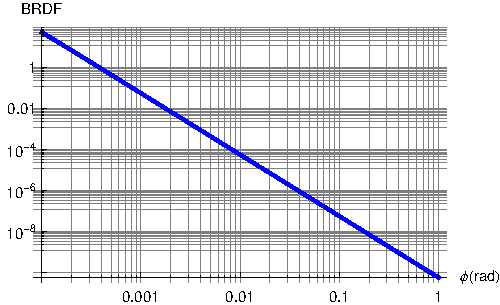
\includegraphics[scale =1]{./Sec_Optics/BRDF-plot.pdf}
\caption{A bidirectional reflectance distribution function (BRDF) of an Advanced LIGO mirror.
The BRDF describes an angular distribution of a scattered light power per
unit solid angle. It was used to assume the scattering efficiency for the
diagonal path scattering process.}
\label{fig:BRDF}
\end{figure}



\begin{figure}
\centering
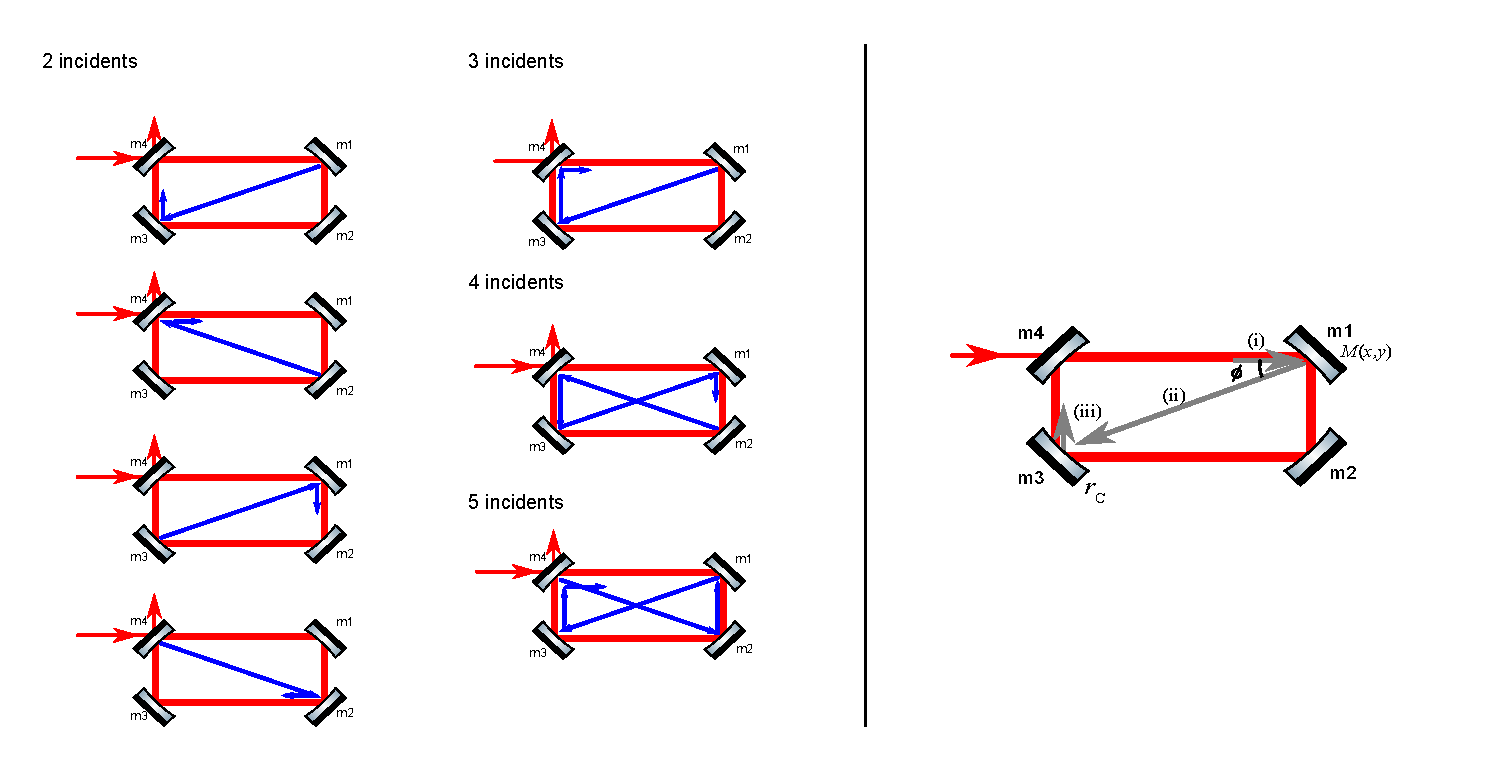
\includegraphics[scale =0.6]{./Sec_Optics/diagonal1.pdf}
\caption{Above left:
Possible routes of the diagonal path scattering.
After the scattered light is emitted by one mirror,
the field propagates along the diagonal path or the shorter path in the rectangular,
then is scattered again or reflected by another mirror,
and finally couples to the main beam. Until coupling into the main beam,
the route is composed of a number of scattering and/or reflection incidents.
Depending on which small angle, large angle scattering, or reflection incident,
one route might have different combinations of spurious paths.
Here, spurious routes with up to 5 incidents were considered.
All possible paths with two incidents are depicted on the left,
while only one example route is shown for 3, 4 and 5 incidents.
Above right:
Example view of small angle scattering and of large angle scattering.
(i)~The scattered light is emitted when the main beam hits m1.
(ii)~The scattered light propagates along the diagonal line.
This incident is considered as the large angle scattering which has a small
scattering efficiency because this diagonal path
is at almost 90 degrees from the main path after the reflection at m1.
(iii)~The scattered field is scattered again at a small angle
with respect to the main beam. This is considered as the small angle scattering
as this path coupling into the main beam is at a very small angle compared with
the reflected path resulting from the diagonal path (from m1).
Depending on whether the scattering angle is large or small,
the corresponding scattering efficiency is taken into account.}
%Upper right panel: scattering process of diagonal path with the large angle
%at the second scattering. Processes~(i) and (ii) are the same as the left panel.
%(iii)~The scattered field is scattered again at a large angle by mirror m3 with its mirror map $M2(x,y)$
%and couples into the Gaussian cavity mode.
%Lower right panel: all the possible incidents of diagonal path II process.
%Similar to the diagonal-I process, $\phi_1$ and $\phi_2$ depend on the paths.
%For example, both $\phi_1$ and $\phi_2$ are small for the gray process,
%on the other hand, $\phi_1$ is large and $\phi_2$ is small for the magenta process.
%The amplitude of the scattered light strongly depends on the scattered angle
%which is summarized in
%Tables~\ref{table:SCcond1} and \ref{table:SCcond2} for all the possible paths.}
\label{fig:diagonal1}
\end{figure}


% path explanation
In the rectangular cavity,
the diagonal lines of the rectangular geometry can become scattered light paths.
When the main beam illuminates a mirror, scattered light fields are produced
by the mirror surface distribution.
The scattered light experiences further scattering or reflection incidents.
There can be many possible spurious paths during this process.
In Fig.~\ref{fig:diagonal1}, all the possible routes with 2 incidents are
shown, while only one example path is shown for other paths
with 3 to 5 incidents. Each route might have one or more spurious paths
because each incident is either from scattering or reflection.
For example, a 3-incident route of m1 - m3 - m4 has
possible paths of m1 (large angle scattering)
- m3 (small-angle and short-path scattering)
- m4 (small angle scattering),
and m1 (large angle scattering) - m3 (reflection)
- m4 (small-angle and short-path scattering),
and m1 (large angle scattering) - m2 (small-angle and short-path scattering)
- m3 (reflection).
Here, we consider such spurious paths with up to 5 incidents.

% counting condition
The total number of possible paths were counted in the following way:
(i) Spurious paths with up to 5 incidents of scatter and/or reflection were considered.
(ii) At the end of the path, the scattered field couples into the main beam in the normal propagating direction. (iii) Direct back scatter was not considered because it is assumed to be smaller than
the coupling in the normal direction at the small angle
(iv) scattered light does not propagate along the long path without coupling into
the main beam.
The total number of the possible spurious paths are
4 paths (all of which are shown in the Fig. \ref{fig:diagonal1}), 10 paths,
12 paths, and 16 paths were found for 3, 4, and 5 incidents, respectively.
To obtain the result, all contributions from all paths are statistically summed.

% small scattering, large scattering, small close scattering
The efficiency of the scattering power is large when the scattering angle,
which is the angle made with the main beam path, is small,
and the efficiency is small when the scattering angle is large.
Therefore, the amplitude of the scattered field depends on the propagation path
and the spurious path.
Here we assume the amplitude using BRDF
which is a function of the scattering angle again.

%After the light field is scattered by the first mirror and propagate the diagonal path,
%there are two possibility to be scattered again at the second mirror.
%The diagonally propagating field is scattered again with small or large scattering angle or large angle,
%as depicted in the left or right panel of Fig.~\ref{fig:diagonal1}, respectively.
%As the incident at a small scattering angle has larger scattering efficiency compared
%with one at the large scattering angle because the most field is scattered to a small angle
%due to the longer spacial frequency of a typical mirror surface, as mentioned above.
%In total, eight paths are considered here.
%For each path, the scattered angles and the coupling direction
%are summarized in Tables~\ref{table:SCcond1} and \ref{table:SCcond2}.

Assuming the scattered field to be a plane wave as a rough approximation,
one can write the scattered field of each path as
\begin{eqnarray}
\label{eq:D1}
%\psi _{\rm sc}(x,y,z) =\frac{\eta (\phi _1) \eta (\phi _2)}{R _d}
%~\exp \Bigl[-i k_0 R_d -2ik_0 M(x,y) +\frac{i k_0 (x^2 +y^2)}{2 r_C} \Bigr]
\begin{split}
\label{eq:D2}
\delta E(x,y,z) =\prod _{n=1}^{N} \eta_n (\phi _n)
\, \exp \Bigl[-i k_0 \bigl\{ R_d +\frac{x^2 +y^2}{2 r_C} \bigr\} \Bigr].
\end{split}
\end{eqnarray}
where $R_d$ is the total path length from the emission point
to the coupling point,
and $r_C$ is the radius of curvature of a mirror when the scattered filed
couples into the cavity, %$M(x,y)$ is the mirror surface map
%of the mirror where the scattered light occurs.
$N$ is the total incidence number,
and $\eta _n (\phi _{n})$ is the amplitude (or efficiency) of the $n$th
incident of scattering or reflection, assumed by BRDF and
the scattering angles.


Substituting Eq.~(\ref{eq:D1}) into Eq.~(\ref{eq:couple}),
the coupling coefficient is derived as
\begin{eqnarray}
%\begin{split}
%X_2= \sqrt{\frac{z_R k_0}{\pi}} \frac{\eta (\phi)}{R_d (z_R +i z_{\rm cav})}
%\int_{\infty}^{\infty} \int_{\infty}^{\infty}
 %\exp \Bigl[-i k_0\bigl\{ R_d+\frac{x^2+y^2}{2 r_C} \qquad \\
%-\frac{x^2+y^2}{(z_{\rm  cav}-i z_R)}+M(x,y)
%\bigr\} \Bigr] {\rm d}x {\rm d}y.
%\end{split}
\begin{split}
X_2= \sqrt{\frac{k_0 z_R}{\pi}} \frac{\prod _{n=1} ^N \eta _n (\phi _n)}{ (z_R +i z _{\rm cav})}
\int_{\infty}^{\infty} \int_{\infty}^{\infty}
\exp \Bigl[-i k_0\bigl\{ R_d+\frac{x^2+y^2}{2 r_C} \qquad \\
-\frac{x^2+y^2}{2(z _{\rm cav}-i z_R)}%+M_1(x,y)+M_2(x,y)
\bigr\} \Bigr] {\rm d}x {\rm d}y.
\end{split}
\end{eqnarray}




%\subsection{Diagonal path scattering II}
%In the rectangular cavity, another coupling process by the diagonal path should be taken into account.
%Similarly to the previous process, the scattered light from one mirror propagate the diagonal path
%as a spherical wave as in the process considered in the previous section.
%Again, spherical waves are possibly overestimate for the propagation,
%but used as a rough approximation.
%Then the scattered field is scattered again by the second mirror
%and couples into the Gaussian cavity mode (upper right panel of Fig.~\ref{fig:diagonal1}).
%As shown in the lower right panel of Fig.~\ref{fig:diagonal1},
%there are four processes possible in a rectangular cavity.

%The light filed after the second scattering is written as
%\begin{eqnarray}
%\begin{split}
%\label{eq:D2}
%\psi _{\rm sc}(x,y,z) =\frac{\eta (\phi _1) \eta (\phi _2)}{R _d}
%~\exp \Bigl[-i k_0 \bigl\{ R_d +\frac{x^2 +y^2}{2 r_C} \\
%+M_1(x,y) +M_2 (x,y) \bigr\} \Bigr].
%\end{split}
%\end{eqnarray}
%where $\phi _1$ is the angle between the main beam and the diagonal path
%when the first scattering, and $\phi _2$ are the angles between the diagonal path
%and the cavity path when the scattered field couples again into the cavity mode.
%%Depending on which path it takes,  $\phi _1$ and  $\phi _2$ are defferent

%Substituting Eq.~(\ref{eq:D2}) into Eq.~(\ref{eq:couple}),
%the coupling coefficient is derived as
%\begin{eqnarray}
%\begin{split}
%X_3= \sqrt{\frac{k_0 z_R}{\pi}} \frac{\eta (\phi _1) \eta (\phi _2)}{R_d (z_R +i z _{\rm cav})}
%\int_{\infty}^{\infty} \int_{\infty}^{\infty}
%\exp \Bigl[-i k_0\bigl\{ R_d+\frac{x^2+y^2}{2 r_C} \qquad \\
%-\frac{x^2+y^2}{2(z _{\rm cav}-i z_R)}+M_1(x,y)+M_2(x,y)
%\bigr\} \Bigr] {\rm d}x {\rm d}y.
%\end{split}
%\end{eqnarray}



\paragraph{(c) Gaussian tail effect}
In the rectangular and bow-tie cavities, the tail of the Gaussian field
may reach the wrong mirror, for example as shown in Fig.~\ref{fig:Gtail} (a),
and is partially reflected. This reflected field couples into the main Gaussian beam.
Note that this is also a simplified picture.
As shown in Fig.~\ref{fig:Gtail} (b), the wave front at the edge of the main field
faces a different direction compared with the wave front at the center
of the beam, therefore, the reflection angle may differ from the main beam path.
However, for a simple estimation, we approximate that
the Gaussian tail field is reflected and directly couples into the main mode.
The rectangular or bow-tie cavity has four fields to be considered
since this process can occur at each mirror.

When a mirror (therefore the coupling point) is a distance $L$ away in the $x$ direction
from the main beam, the coupling field is written as
\begin{eqnarray}
\delta E (x,y,z) =E _c  (x+L _s,y,z _{\rm sc}).
\end{eqnarray}

The coupling coefficient is
\begin{eqnarray}
\begin{split}
X_4=\frac{-k_0 z_R}{\pi (i z _{\rm cav}+z_R) (iz _{\rm sc}-z_R)}\qquad \qquad \qquad \qquad \qquad \qquad \\
\int_{\infty}^{\infty} \int_{\infty}^{\infty}
\exp \Bigl[-i k_0 \Bigl\{
\frac{x^2+y^2}{2(i z_R-z _{\rm cav})}+\frac{(L_s+x)^2+y^2}{2(i z_R-z _{\rm sc})} \Bigr\}
\Bigl]  {\rm d}x {\rm d}y.
\end{split}
\end{eqnarray}


\begin{figure}
\centering
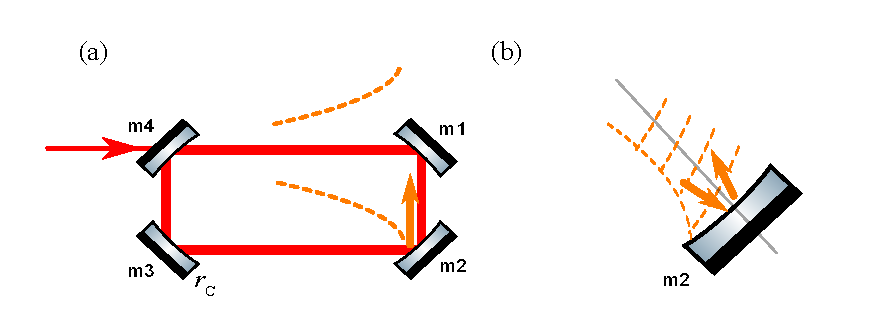
\includegraphics[scale =1]{./Sec_Optics/Gtail.pdf}
\caption{(a) An example dagram of the Gaussian tail effect. This process will occur at each mirror
in the rectangular and bow-tie cavities.
(b) Detailed diagram of the wave fronts at the tail of Gaussian field.
In the picture, the incident angle and the reflection angle
is slightly different from the approximated picture (a).}
\label{fig:Gtail}
\end{figure}


\paragraph{Numerical evaluation}

In order to numerically calculate the coupling coefficient,
we assume that the round trip of a cavity is about 10 km,
and the waist position of the laser beam is at the middle point of the round trip
for all the geometries, as shown in Fig.~\ref{fig:geo-summary}.
The triangular cavity is an isosceles triangle with two 5 km arms and with a 1 m base,
and the beam waist is at the middle of the short path.
The rectangular cavity has long and short paths of 5 km and 1 m respectively,
and the beam waist is at m2 in Fig.~\ref{fig:geo-summary}.
The bow-tie cavity has four paths of 2.5 km
and the separation between the closer mirrors is assumed to be 1 m.
For mode-matching, each mirror was assumed to be either flat
or to have a radius of curvature $r_C$.
%ET fake mirror maps simulated using a sum of
%Zernike polynomials with maximum 1 nm amplitude were used \cite{bond10}.


\begin{figure}
\centering
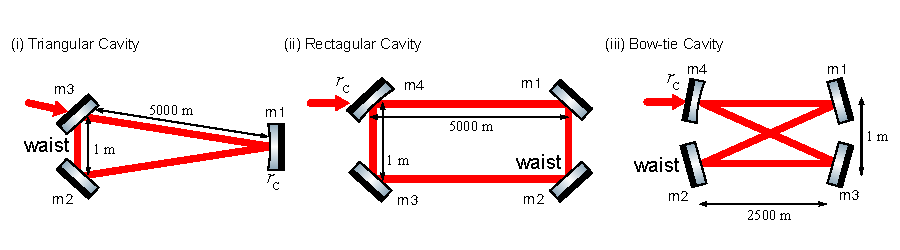
\includegraphics[scale =1]{./Sec_Optics/geo-summary.pdf}
\caption{Cavity designs used for the numerical calculation.
The cavities have a round trip length of approximately
10 km, and a beam waist at the middle point of the path.}
\label{fig:geo-summary}
\end{figure}


$\bullet$  Direct back scattering:
Fig.~\ref{fig:scat-plot-1} shows the plot of $X_1$ over the mirror angle $\alpha$
for four coupling locations ($z$=1, 1000, 2500, {\rm and} 5000).
$X_1$ strongly depends on the angle between
the mirror normal and the propagation direction of the beam, $\alpha$.
The coupling coefficient rapidly approaches zero
when the angle is larger than $10^{-3}$ degrees.
This is because the coupling between the two fields is
very small when the wavefront of one field is delayed
by the mirror surface with the incident angle while the other field is not delayed.
Since the mirror angles of all the ring cavities have much larger $\alpha$,
the direct back-scattering is negligible in ET cavities
although arbitrary scattering angles
(i.e. arbitrary scattering efficiencies $\eta$) are considered here.
%However one has to be careful not to have mirror surface structures
%which may generates additional scattering light.

%numerical evaluation will show that no direct back scattering effect
%is expected at the detection port.


\begin{figure}
\centering
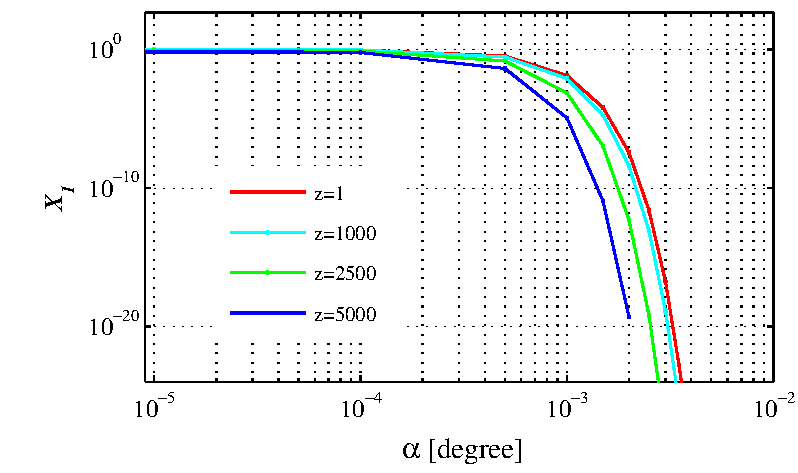
\includegraphics[scale =.7]{./Sec_Optics/scat-plot-1.pdf}
\caption{The coupling factor $X_1$ (direct back scattering) over the mirror angle
where the scattering process occurs.
The coupling factor rapidly goes to zero after $10^{-3}$ degrees.}
\label{fig:scat-plot-1}
\end{figure}

$\bullet$ Diagonal path scattering:
From the assumption using BRDF and the scattering angles
when the longer and the shorter path lengths of the rectangular cavity
are 10 km and 1 m respectively,
the amplitude of the small angle scatter is
$\eta (\phi _{\rm s})=3.8 \times 10^{-8}$,
of the large angle scatter is $\eta (\phi _{\rm s})=7.5 \times 10^{-6}$,
and of the small-and-short scatter is $\eta (\phi _{\rm SS})=4.1 \times 10^{-5}$.
%(coupling coefficient varies depending on the coupling point.)
Adding the coupling coefficients of all the possible paths
up to 5 incidents, the total coupling coefficient was calculated
to be $4.7 \times 10^{-11}$ when the intra cavity power is normalised as unity.
Therefore, one should be careful to consider the scattering field propagating
along the diagonal paths in the rectangular cavity.
In order to block the diagonal paths, placing baffles
inside the rectangular geometry will be useful
to prevent the scattered light coupling into the cavity mode.

%Taking the statistical sum of the eight scattered fields,
%the total amplitude of the scattered filed is $2.5 \times 10^{-12}$,
%while the laser power is normalised to be unity at each mirror.

$\bullet$ Gaussian tail effect:
The Gaussian tail effect is found to be negligible
with the optical parameters considered here.
In numerical simulations a length of 1 m for the shorter paths
in rectangular or bow-tie cavities was found to be sufficient
for the effect to be negligible.
%Although this length should be careful not be too close.


%\subsection{Summary}
Table~\ref{table:summary} shows a summary of the numerical evaluation.
The two-mirror cavity is the best configuration from the scattered-light
point of view because there are no spurious paths in the geometry.
For the other three configurations,
the direct back scattering and the Gaussian tail effect were found to be negligible.
One should be careful to consider the scattering field propagating
along the diagonal paths in the rectangular cavity.
If this geometry is to be used, the placement of baffles
inside the rectangular geometry will be necessary
to prevent the scattered light from propagating along the paths.



\begin{table}
\begin{center}
\begin{tabular}{|c|c|c|c|c|}
\hline
Type        & direct-back scattering &  Diagonal & Gauss. Tail \\ \hline
Two-mirror   &   N/A  &  N/A   & N/A   \\ \hline
Triangular     & $0$ &  N/A    & N/A   \\ \hline
Rectangular  &  $0$ &  $4.7\times 10^{-11}$ & 0\\ \hline
Bow-tie        &  $0$ &  N/A  & 0    \\ \hline
\end{tabular}
\caption{Summary of the scattering process for each geometry without
an amplification factor of the cavity.
The numbers are in amplitudes while the light power is normalised
to be unity inside the cavity.}
\label{table:summary}
\end{center}
\end{table}


\FloatBarrier
\subsubsection{Noise couplings}\label{app:phsnoise}
%We should consider\dots
%\begin{itemize}
%\item{Frequency noise}
%\item{Phase noise due to displacement noise}
%\item{Length stabilization}
%\item{Alignment noise/pointing?}
%\item{Scattering}
%\end{itemize}

In this section several noise mechanisms that potentially limit the detected squeezing levels are discussed. First, we discuss the effect of phase noise in the squeezing path. Assuming a self-homodyning readout (DC readout) of the interferometers  signal field, the DC part of the interferometer output field serves as local oscillator. The quadrature of the signal field that is read out is determined by its relative phase with regard to this local oscillator. In order to reduce the quantum noise of this measurement, the relative phase of the injected squeezed field needs to be chosen such that the squeezed quadrature coincides with the readout quadrature. This required phase relation gets disturbed due to e.g.\ vibrating optical components in the squeezing path (displacement noise) or residual high frequency phase modulations that probably will be required for control purposes.  If the measurement time is greater than the period of the phase jitter period, the homodyne read out is not a pure measurement of a certain quadrature   $\zeta$ (e.g.\ the squeezed quadrature) but the integral over some span of $\zeta+\delta \zeta$. In this case, a certain fraction of the noise in the anti-squeezed quadrature is mixed into the measurement that was intended to be a measurement of the squeezed quadrature. It is obvious, that such a \textit{phase diffused squeezed state}  results in a degraded squeezing level.  Accordingly, an upper limit for the overall tolerable phase noise in the squeezing path needs to be deduced with regard to the targeted quantum noise reduction of 10\,dB.

The influence of phase noise on the squeezed field can be nicely illustrated by the accordant Wigner functions. We start from the Wigner function of a squeezed state that has a certain orientation (determined by the quadrature angle  $\varphi$) in phase-space. It is  given by
\begin{equation}
W(X_{1,\varphi},X_{2,\varphi}, \varphi) = \frac{1}{2\pi\sqrt{V_sV_a}}\exp\left[-\frac{X_{1,\varphi}^2}{2V_s}-\frac{X_{2,\varphi}^2}{2V_a}\right]\,.
\end{equation}
Here $V_s$ and $V_a$ denotes the variances in the squeezed and anti-squeezed quadrature, respectively (e.g.\ for a pure 10\,dB squeezed state  $V_s=0.1$ and $V_a=10$ if normalised to the variance of the vacuum state $V_{\rm{vac}}=1$).  The orientation in phase-space is accounted for by setting
\begin{eqnarray}
X_{1,\varphi} &=& X_1\cos(\varphi) - X_2\sin(\varphi)\\
X_{2,\varphi}  &= &X_1\sin(\varphi) + X_2\cos(\varphi)\,.
\end{eqnarray}%

Here, the local oscillator serves as reference for the phase-space with its amplitude ($X_1$) and phase quadrature ($X_2$). The corresponding probability distribution in the amplitude quadrature ($X_1$) can be obtained from the Wigner function by integrating over $X_2$. One obtains
\begin{eqnarray}
P_{X_1} &=& \int\limits_ {-\infty}^{\infty}W_d(X_1,X_2)dX_2\\
&=&\frac{1}{{\sqrt{2\pi V_{X_1}(\varphi)}}}\exp\left[-\frac{X_1^2}{2V_{X_1}(\varphi)} \right]\,.
\end{eqnarray}

with the variance of the amplitude quadrature
\begin{eqnarray}
V_{X_1}(\varphi) &=& V_s\cos^2(\varphi) + V_a\sin^2(\varphi)\\
&=&\frac{1}{2}\left[V_s+V_a+(V_s-V_a)\cos(2\varphi)\right]\,.
\end{eqnarray}
Now, to describe a phase-diffused squeezed state, the quadrature angle $\varphi$ needs to be replaced by a probability density for the phase denoted as $\Phi(\varphi)$. Then, the Wigner function is given by
\begin{equation}
W_d(X_1,X_2) =\int \Phi(\varphi) W_d(X_1,X_2, \varphi)d\varphi\,.
\end{equation}

Again, the corresponding probability distribution in the amplitude quadrature ($X_1$) can be obtained from the Wigner function by integrating over $X_2$
\begin{equation}
P_{X_1,d} = \int\limits_ {-\infty}^{\infty}W_d(X_1,X_2)dX_2 \,.
\end{equation}
Accordingly, the variance of a phase-diffused squeezed state is given by
\begin{equation}
V_{X_1,d} = \int\limits_{-\infty}^{\infty}\Phi(\varphi)V_{X_1}d\varphi\,\Leftrightarrow  \int\limits_{-\infty}^{\infty}P_{X_1,d}X_1^2dX_1\,.\label{eq:varsqzphsdiff}
\end{equation}

\begin{figure}
\centering
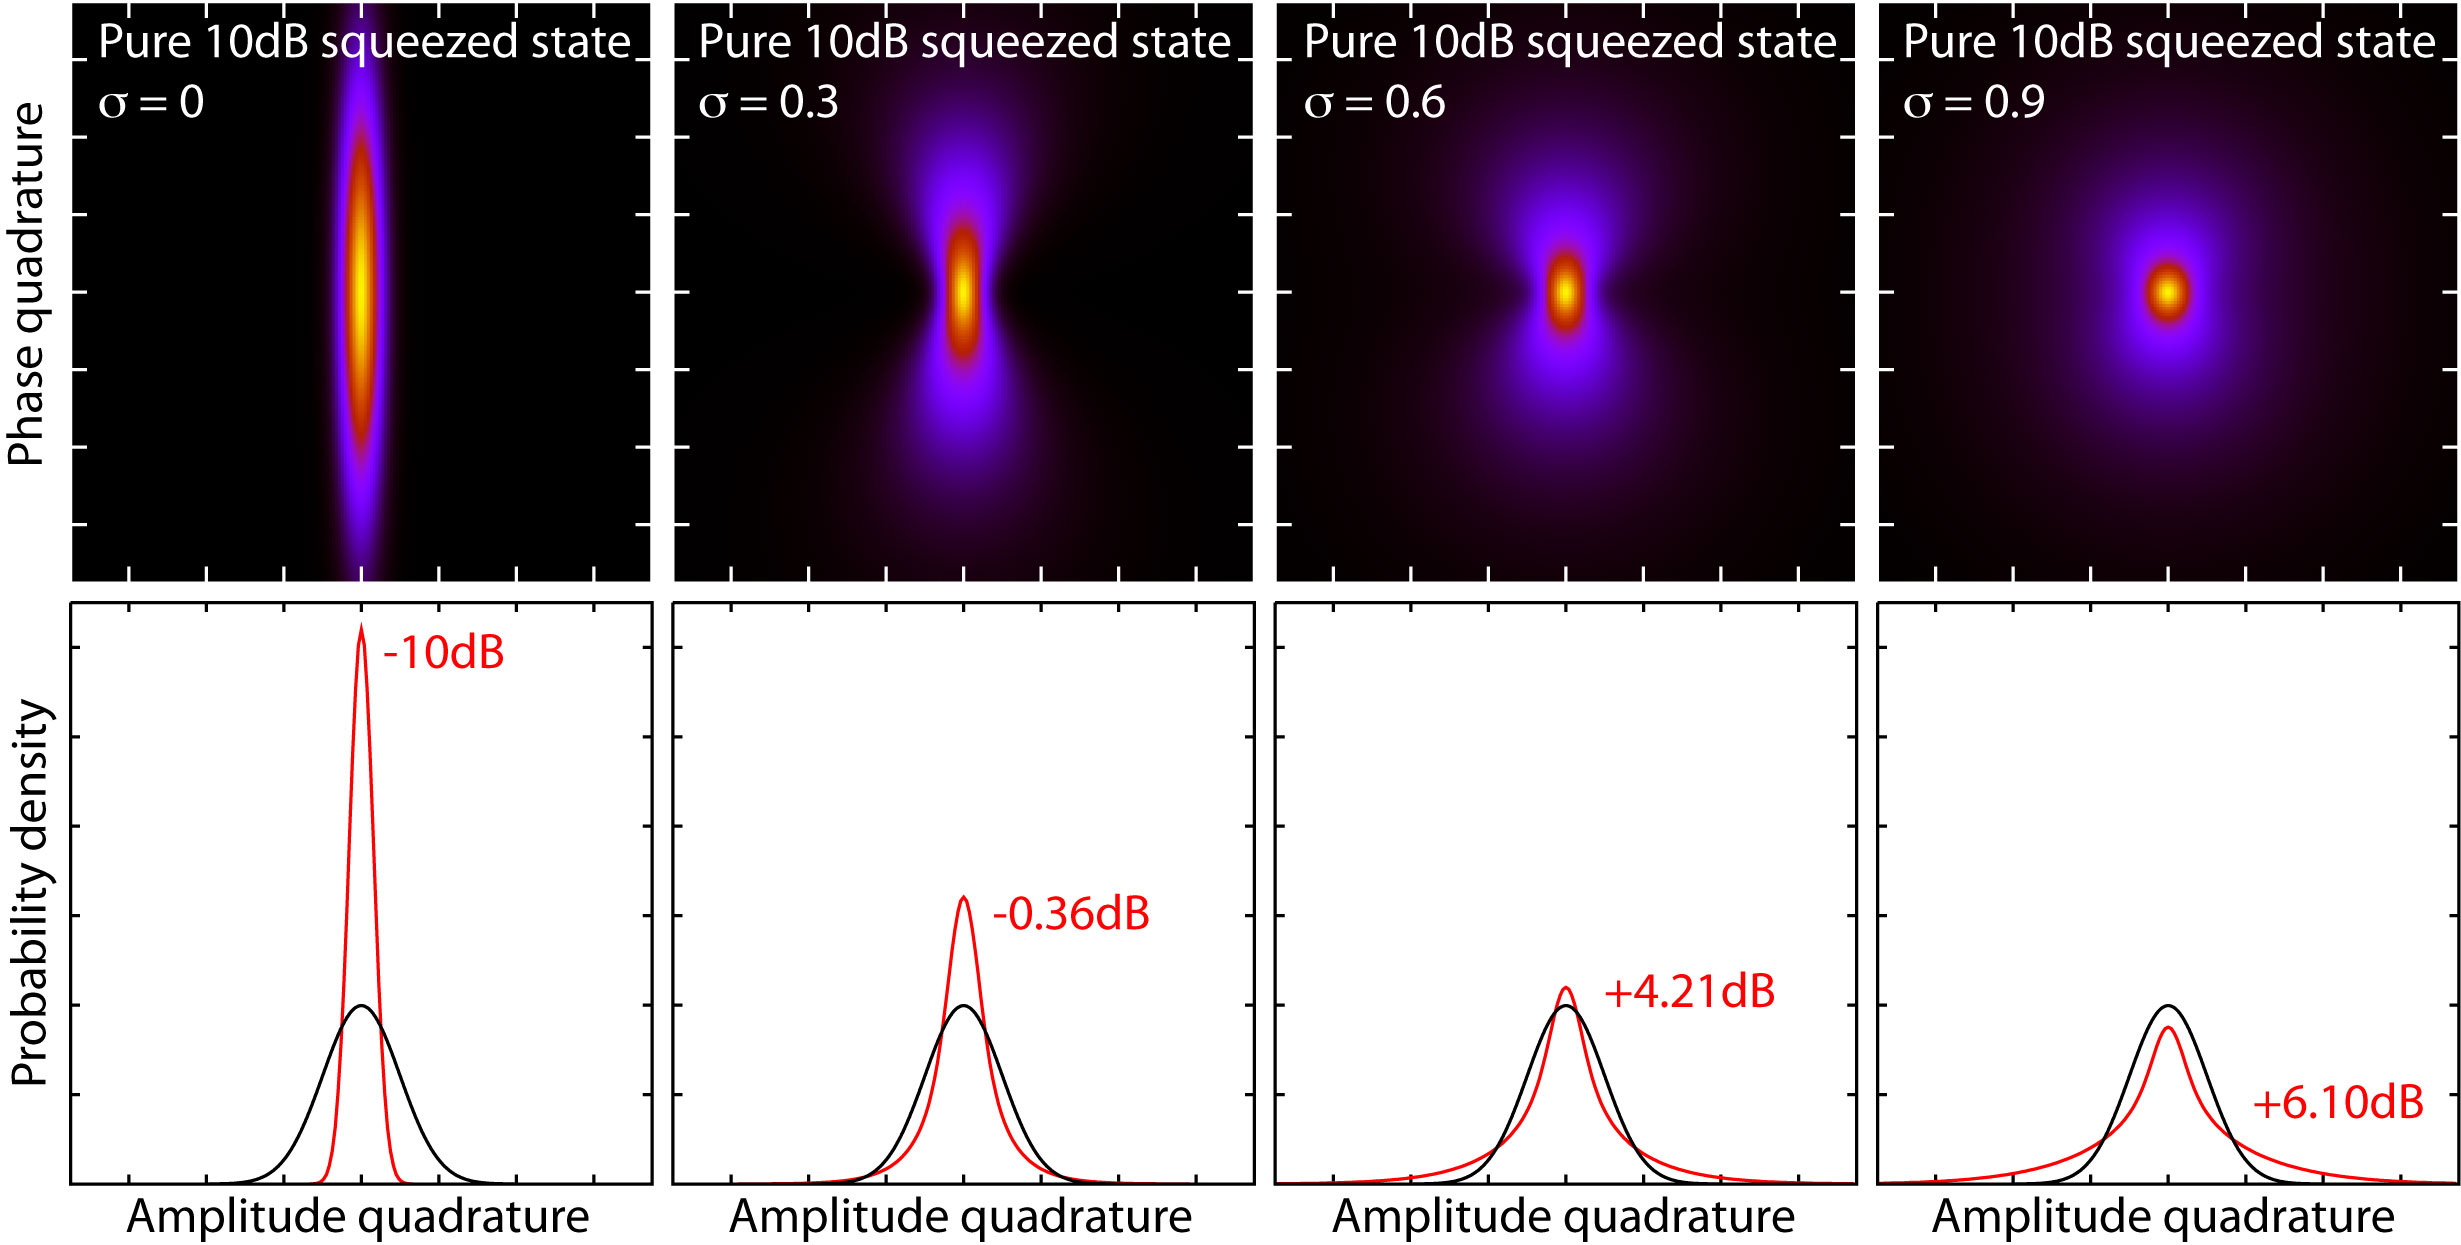
\includegraphics[scale=0.77]{./Sec_Optics/Wig_10dB_all.jpg}
\caption{Illustration of the influence of a Gaussian distributed phase noise on the squeezed state. \textbf{Top:} Wigner functions for phase noise  with a standard deviation $\sigma$ of 0, 0.3, 0.6, 0.9\,rad. The initial, pure squeezed state was assumed with 10\,dB. \textbf{Bottom:} The probability distribution of the phase diffused squeezed states and the corresponding squeezing levels (red curves and red labels, respectively) in the  amplitude quadrature ($X_1$).  For comparison, the distribution of a vacuum state is shown (grey curves).}
\label{fig:phasediffusedSQZ}
\end{figure}

In Fig.~\ref{fig:phasediffusedSQZ} four Wigner functions  (top) and the corresponding probability distribution in the $X_1$-quadrature (bottom) are shown. We assumed a Gaussian-distributed phase noise, i.e,
\begin{equation}
\Phi(\varphi) = \frac{1}{\sqrt{2\pi\sigma^2}} \exp\left(-\frac{\varphi^2}{2\sigma^2}\right)\,.
\end{equation}
Note that no specific assumptions on the spectral distribution of the phase noise have been made. In order to deduce the value of the variance of $\varphi$ from a measured spectrum of the phase noise the integral over the full observation bandwidth has to be taken.

We have considered phase noise with  a standard deviation $\sigma$ of 0 (no phase noise), 0.3, 0.6 and 0.9\,rad (from left to right in Fig.~\ref{fig:phasediffusedSQZ}). The initial squeezed state (left figures) was assumed with $V_s=0.1$ and $V_a=10$, i.e.\ as a pure 10\,dB squeezed state. The degradation of the squeezing level due to phase noise becomes obvious from the comparison with the probability distribution of a vacuum state (grey traces in the bottom graphs). The probability distributions are labelled with the corresponding squeezing level. For strong phase noise  the initial squeezing is destroyed and the noise in the amplitude quadrature is even enhanced when compared to the vacuum noise (shot noise).





\begin{figure}[!h]
\centering
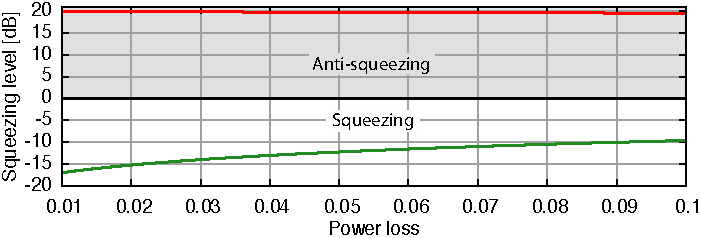
\includegraphics[scale=1]{./Sec_Optics/SQZ-20dB-losschartAI.pdf}
\caption{The degradation of the squeezing and anti-squeezing levels due to optical loss for an initially pure (no loss) 20\,dB squeezed state.}
\label{fig:20dBlosschart}
\end{figure}

The illustration in Fig.~\ref{fig:phasediffusedSQZ} implies that the larger the anti-squeezing level, the larger the effect of phase noise. In fact, in order to achieve the targeted quantum noise reduction of 10\,dB, a squeezed light source needs to be utilised that generates considerably more than 10\,dB (anti-)squeezing to compensate for possible loss. If an overall optical loss of up to 10\,\% in the squeezing path (including 1\,\% loss in the squeezed light source itself) is assumed, an initially pure 20\,dB squeezed state needs to be generated. The degradation of the squeezing (and anti-squeezing) level with optical loss is shown in Fig.~\ref{fig:20dBlosschart}. Whereas the squeezing level is strongly affected by optical loss, the anti-squeezing level is not considerably reduced. Considering an overall optical loss of 10\,\% the squeezing level is reduced from 20\,dB to about 9.6\,dB, but the anti-squeezing level is still about 19.5\,dB. In Fig.~\ref{fig:phasediffusedSQZ20dB} the effect of phase noise on an initial 20\,dB squeezed state is illustrated, for which optical loss of 1\,\%, 3\,\%, 5\,\% and 10\,\% was considered. Here the phase noise was assumed with a standard deviation of $\sigma=0.3\,rad$. Again,  the top graphs show the Wigner functions and the bottom graphs the probability distribution in the amplitude quadrature. Here, in each case three traces are plotted. The red trace is the distribution of the phase diffused squeezed state and the black one that of a vacuum state. The grey curves correspond to the distribution without phase noise, i.e.\ the degradation of the squeezing level only due to the considered optical loss can be deduced. Again, it can be seen that the high phase noise destroys the squeezing. In each case, the resulting noise level is considerably enhanced when compared to the shot noise level. Please note that although the squeezing levels in the undisturbed case are $\geq$10\,dB, the high anti-squeezing level of almost 20\,dB leeds to higher noise levels when compared to the pure 10\,dB squeezed state (refer to Fig.~\ref{fig:phasediffusedSQZ}). I.e.\ in presence of phase noise the achievable squeezing level can be  optimized by reducing the anti-squeezing (and thus the squeezing) generated by the squeezed light source. On the other hand, that means that in presence of considerable phase noise a compensation of optical loss in the  squeezing path is not possible by enhancing the  squeezing (and thus the anti-squeezing) generated in the squeezed light source.

\begin{figure}
\centering
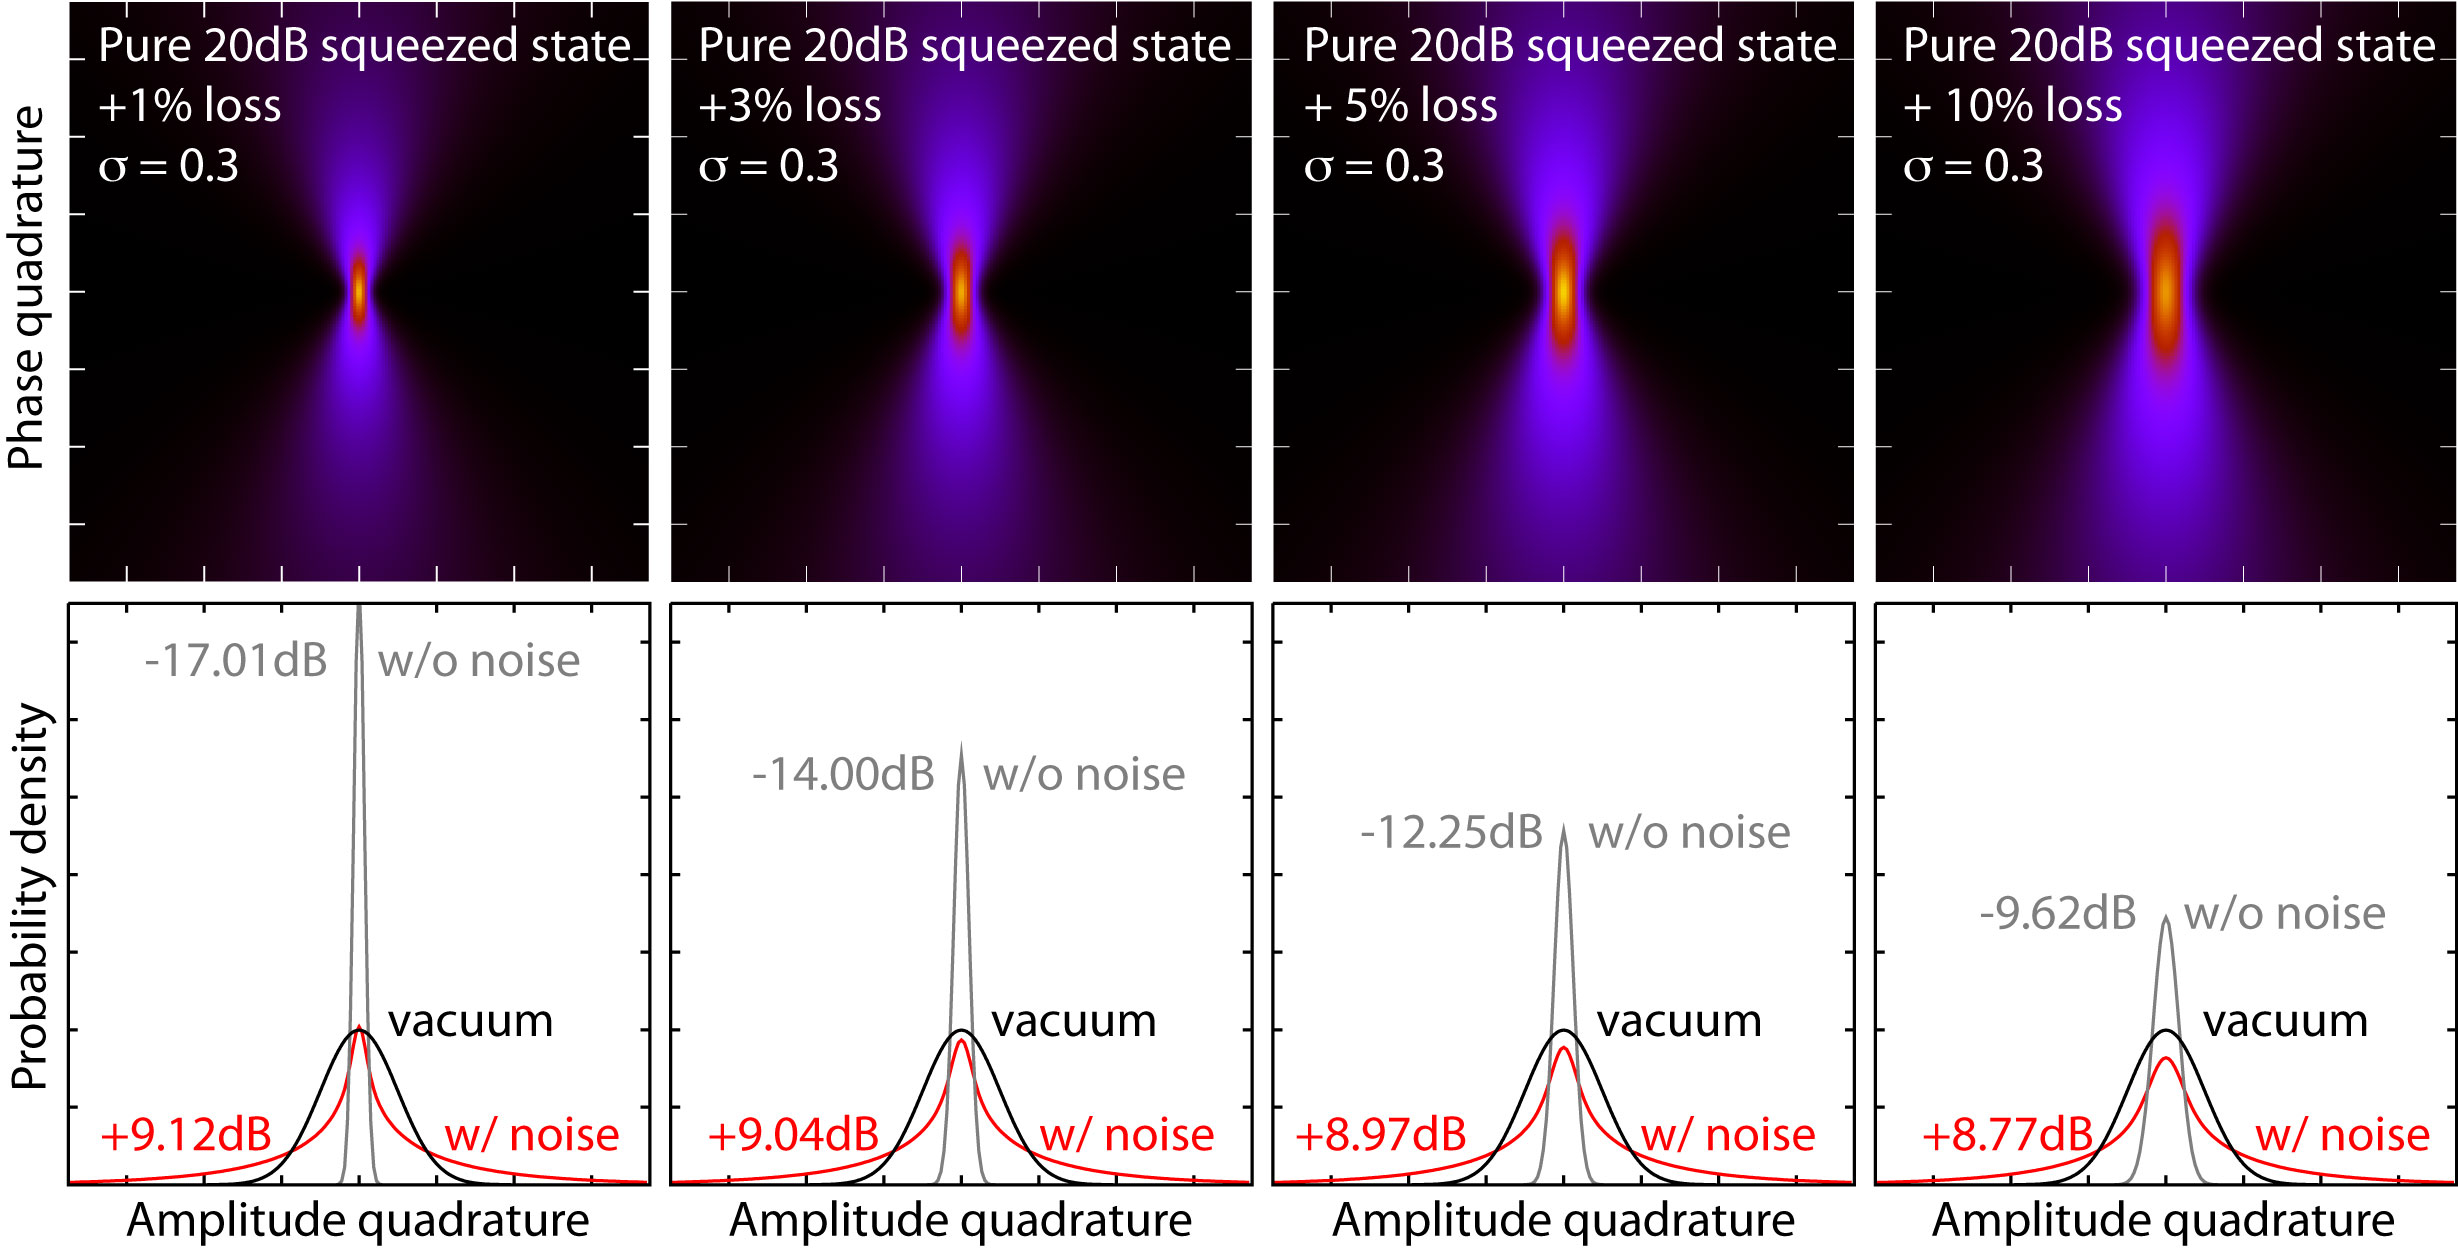
\includegraphics[scale=0.77]{./Sec_Optics/Wig_20dB_loss.jpg}
\caption{The degradation of the squeezing and anti-squeezing levels due to optical loss for an initially pure (no loss) 20\,dB squeezed state.
\textbf{Top:} Wigner functions for phase noise  with a standard deviation $\sigma$ of 0.3\,rad and losses of 1\%,3\%,5\%, and 10\%. The initial, pure squeezed state was assumed with 20\,dB. \textbf{Bottom:} The probability distribution of the phase diffused squeezed states and the corresponding squeezing levels (red curves and red labels, respectively) in the  amplitude quadrature ($X_1$).  For comparison, the distribution of a vacuum state (black curves) and the squeezed state without phase noise but with optical losses (grey curves) is shown.}
\label{fig:phasediffusedSQZ20dB}
\end{figure}


In the previous investigation comparatively high values for the phase noise was considered for illustration purpuses. Such high values are not expected to be present in a realistic experimental environment. However, the upper limit for the overall phase noise in the squeezing path depends on the squeezed state, that is generated by the squeezed light source. Table~\ref{tab:phsnoiselimit} lists the allowed phase noise (i.e.\ its standard deviation) for several conditioned squeezed states. The states were constituted for several values of the optical power  loss $l^2$ such that the  squeezing level without phase noise is 10\,dB. The required squeezing  that needs to be generated inside the squeezed light source can be calculated according to
\begin{equation}
V_s = 0.1 -l^2\hspace{11pt}\text{and}\hspace{11pt}V_a = \frac{1}{V_s}.
\end{equation}
We relate the upper limit $\sigma_{\rm max}$ for the phase noise to a squeezing level that is reduced to 9\,dB due to the phase noise. As the phase noise is assumed to be Gaussian-distributed with zero mean, Eq.~(\ref{eq:varsqzphsdiff}) can be solved giving
\begin{equation}
V_{X_1,d} = \frac{1}{2}\left[V_s+V_a+(V_s-V_a)\exp\left(-2\sigma^2\right)\right]\,.\label{eq:varianzsqzpn}
\end{equation}
Soving Eq.~(\ref{eq:varianzsqzpn}) for $\sigma$ yields
\begin{equation}
\sigma = \sqrt{-\frac{1}{2}\log\left[\frac{2V_{X_1,d}-V_s-V_a}{V_s-V_a}\right]}\,.
\end{equation}
From this equation the tolerable phase noise characterised  by $\sigma_{max}$ can be calculated for the targeted variance  $V_{X_1,d}=0.1$ and squeezing level of 10\,dB, respectively. It turns out that for realistic values of squeezing and anti-squeezing the squeezing phase will have to be stabilised with respect to the phase of the local oscillator of the interferometer, but the phase stability requirements are fairly easy to fulfil. The resulting requirements on the stability of the length of the filter cavity are increased roughly by the finesse of the cavity, but are also rather easily met.


\begin{table}
\begin{center}
\begin{tabular}{rrrrr}
\hline
%\hline
optical loss [\%]& initial squeezing [dB] & squeezing [dB] & anti-squeezing [dB] & $\sigma_{\rm max} [rad]$ \\
\hline
1 & -10.41 & -10 & 10.37 & 0.049\\
3 & -11.41 & -10 & 11.29 & 0.044\\
5 & -12.79 & -10 & 12.58 & 0.038\\
9 & -19.59 & -10 & 19.19& 0.018 \\
10 & $-\infty$ & -10 & $\infty$ & 0\\
20 & $-\infty$ & -6.99 & $\infty$ & 0\\
\hline
%\hline
\end{tabular}
\end{center}
\caption{The table lists  the squeezing and anti-squeezing levels and the tolerable maximum mean phase noise for several values of optical loss.}
\label{tab:phsnoiselimit}
\end{table}

%From the tolerable $\sigma_{\rm max}$ the following requirements can be deduced:
%\begin{itemize}
%\item{the allowed displacement noise in the  filter cavities}
%\item{the requirements for the filter cavity length stabilization}
%\item{the requirements on frequency noise of the squeezed light source related to main interferometer beam}
%%\item{Alignment noise/pointing?}
%%\item{Scattering}
%\end{itemize}
\FloatBarrier

%\subsubsection{Length control of the filter cavities}
%We will analyse
%\begin{itemize}
%\item{the realisation of a locking scheme without introducing too much optical loss (due to pick-off mirrors needed for detection ports). }
%\item{the potential of using the orthogonal polarisation for error signal generation.}
%\item{the restrictions to RF sidebands. They need to be in the same mode as the squeezing, therefore generated in the squeezer by means of the coherent control beam.}
%\item{RF Frequencies. Needs to be reflected at least at the OMC in order not to spoil the IFO.}
%\item{A ring -vs- a linear filter cavity design. If linear filter cavities are used additional Faraday rotators are required.}
%\item{Put the above just as note at a certain point, e.g. within the noise section}
%\end{itemize}


